\section{Materials and Methods}
\subsection{Experimental Setup}
To obtain energies up to $\SI{400}{\kilo\electronvolt}$, a single
Van-de-Graaff accelerator \cref{fig_setup3} was used. The variety of incomming
beam particles was limited by the source (a flask of hydrogen gas connected to
the accelerator tank), which was stationary and not changed. Therefore, we only
concider incomming ions $\mathrm{H^+}$ and $\mathrm{{H_2}^{+}}$. 
%
\begin{figure}[t]
    \centering
    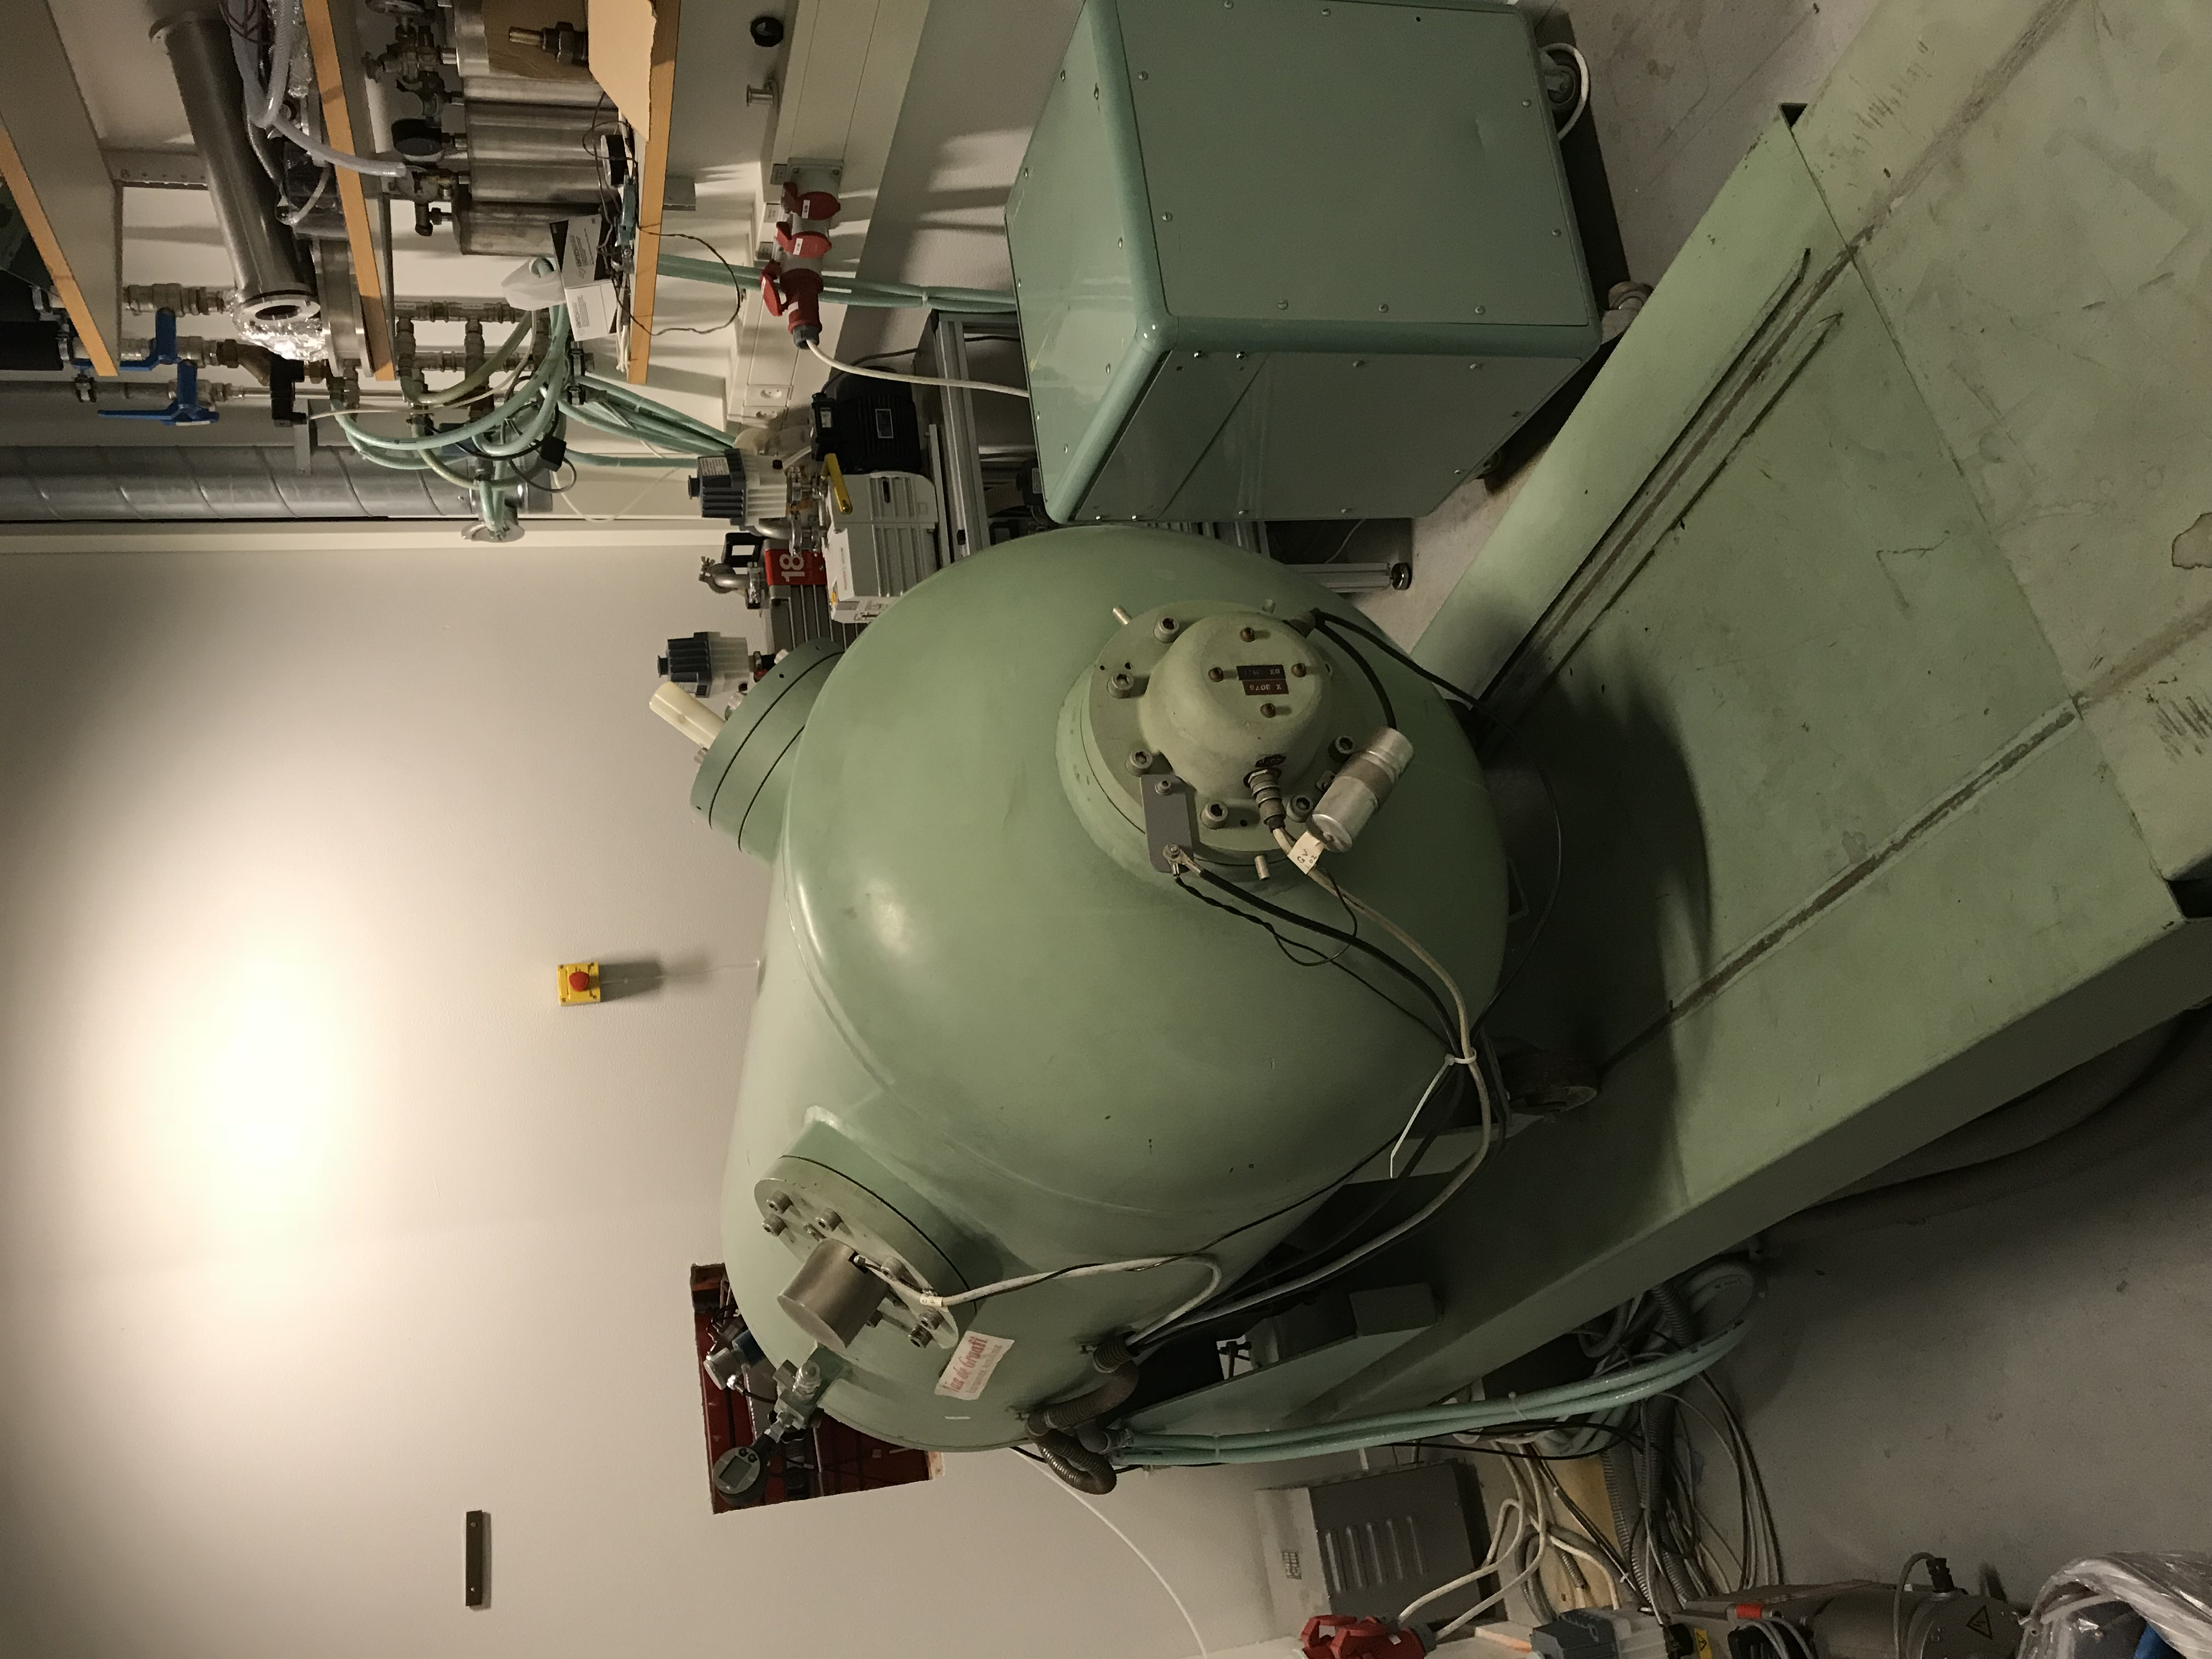
\includegraphics[angle=-90, trim={35cm, 0cm, 27cm, 0cm}, clip,  width=0.99\columnwidth]{setup3}
    \caption{The Van-de-Graaff accelerator.}
    \label{fig_setup3}
\end{figure}
%
Acceleration of the ions was controllable by changing the voltage drop on the
dashboard \cref{fig_setup2} and thus also adjusting the kinetic energy of the
incoming beam. This will be described further later on (see section Procedure).

The beamline was placed in an angle relative to the accelerator
\cref{fig_setup1}. By changing the magnetic field strength of the
electromagnet, one could choose which of the two possible incoming ions were
deflected into the beamline and thus directed towards scattering on the target material at the end of the beamline. 
The motion of a charged particle in a magnetic field is governed by the Lorentz
force law, and as the trajectory of the motion is traced as part of a circle,
one obtains the necesarry equality for the motion to be\footnote{Concepts as
forces and spatial confinements to circular paths is meaningfull in the
classical regime. This is not the case for a fully relativistic and quantum
mechanical description.}

\begin{equation}
F_|m| = QvB = F_|cp| = \frac{mv^2}{r}.
\end{equation}
From this a ratio between the two magnetic fields needed for the respective
ions is
\begin{align}
    R_|B| = & \frac{B({\mathrm{H_2}^+})}{B(\mathrm{H^+})} =
    \frac{m({\mathrm{H_2}^+})
    v({\mathrm{H_2}^+})}{m(\mathrm{H^+})v(\mathrm{H^+})}\\
    & 2 \frac{v({\mathrm{H_2}^+})}{v(\mathrm{H^+})} = \sqrt{2},
\end{align}
%
where it has been assumed that the mass of the two ions are related by
$m(\mathrm{{H_2}^+}) = 2m(\mathrm{H^+}) $ and the speed of each ion is given as
$v(\mathrm{X}) = \sqrt{\frac{2E}{m(\mathrm{X})}}$.
%
Given one of the magnetic fields, the other is determined from this ratio
factor. The following magnetic field strengths were used:
%
\begin{equation}
    B(\mathrm{H^+}) = \SI{1070}{\gauss} \quad B(\mathrm{{H_2}^+}) = \SI{1513}{\gauss}
\end{equation}
%
Conclusively, by changing the magnetic field strength, one changes the
incomming ion. However, the magnetic field strength can change over time scales
of a meassurement. This is a consequence of heating. The iron core is heated
mechanically and thus its magnetic permeability changes. Also, the wire is
heated electrically. As the resistance increases with temperature the
current at a given potential will decrease; giving a lower effective magnetic
field.

%
\begin{figure}[t]
    \centering
    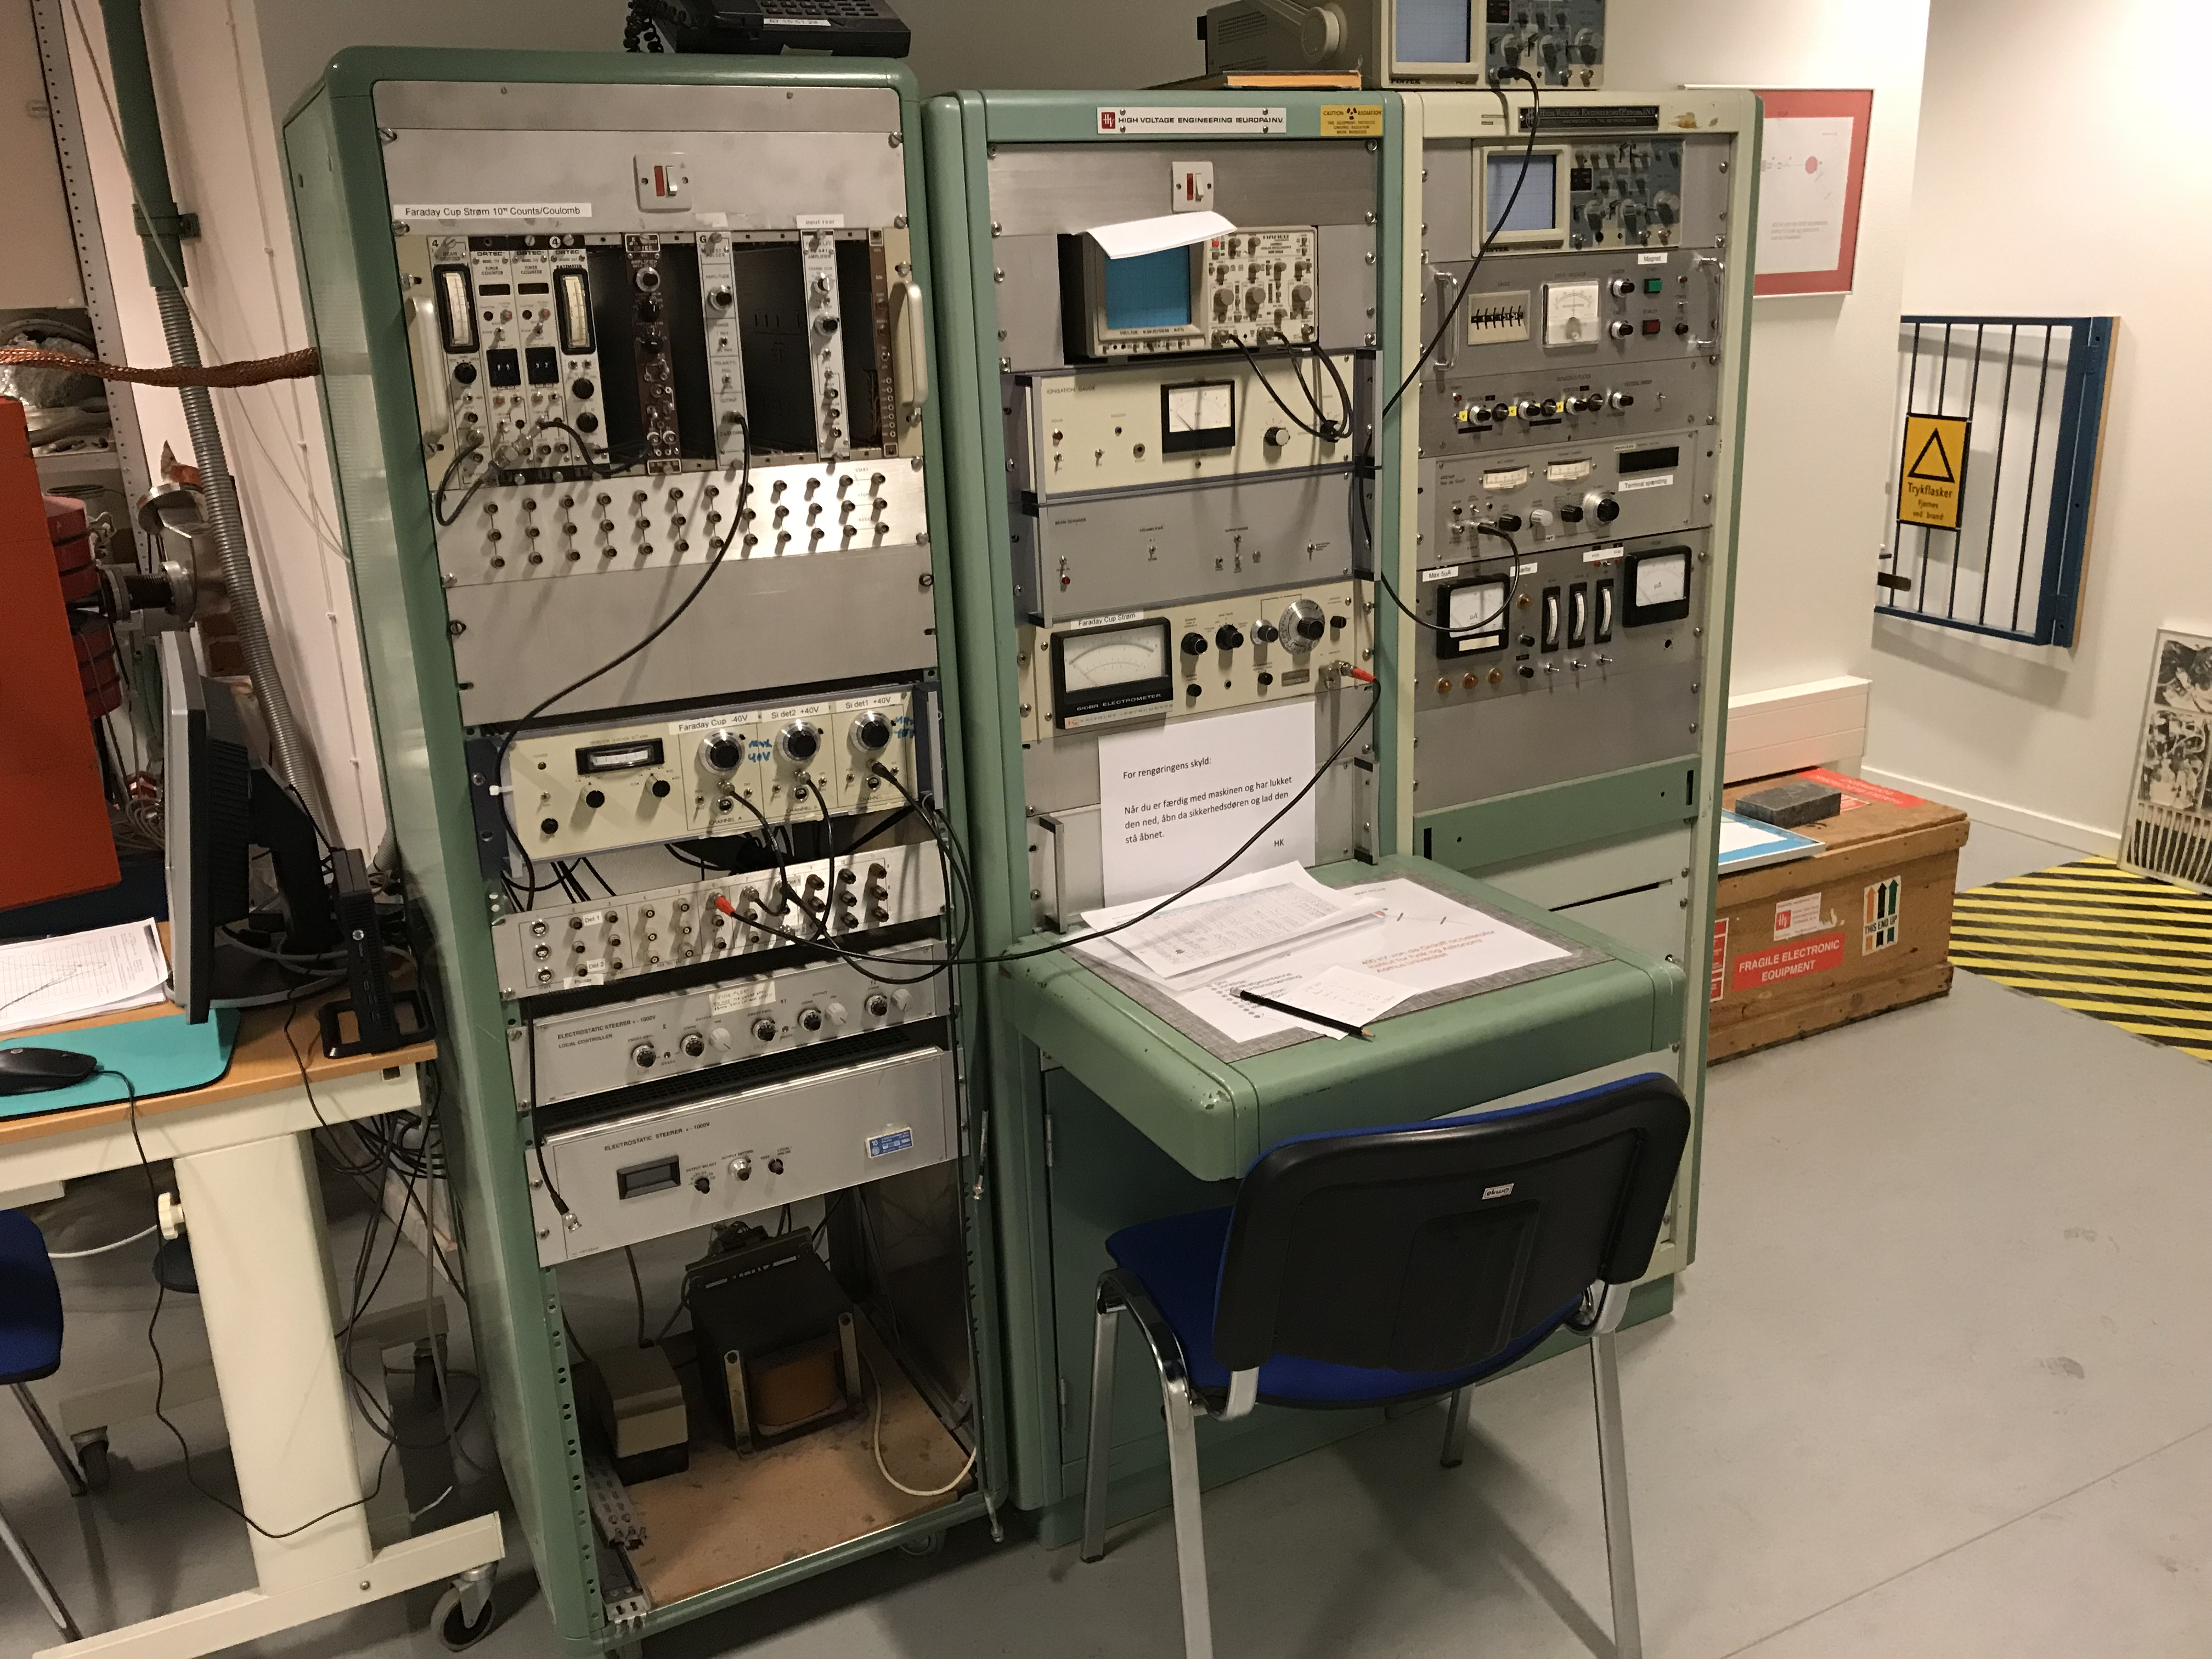
\includegraphics[width=0.99\columnwidth]{setup2}
    \caption{Overview of dashboard. Closer graphics are seen in the Procedure.}
    \label{fig_setup2}
\end{figure}
%
\begin{figure}[t]
    \centering
    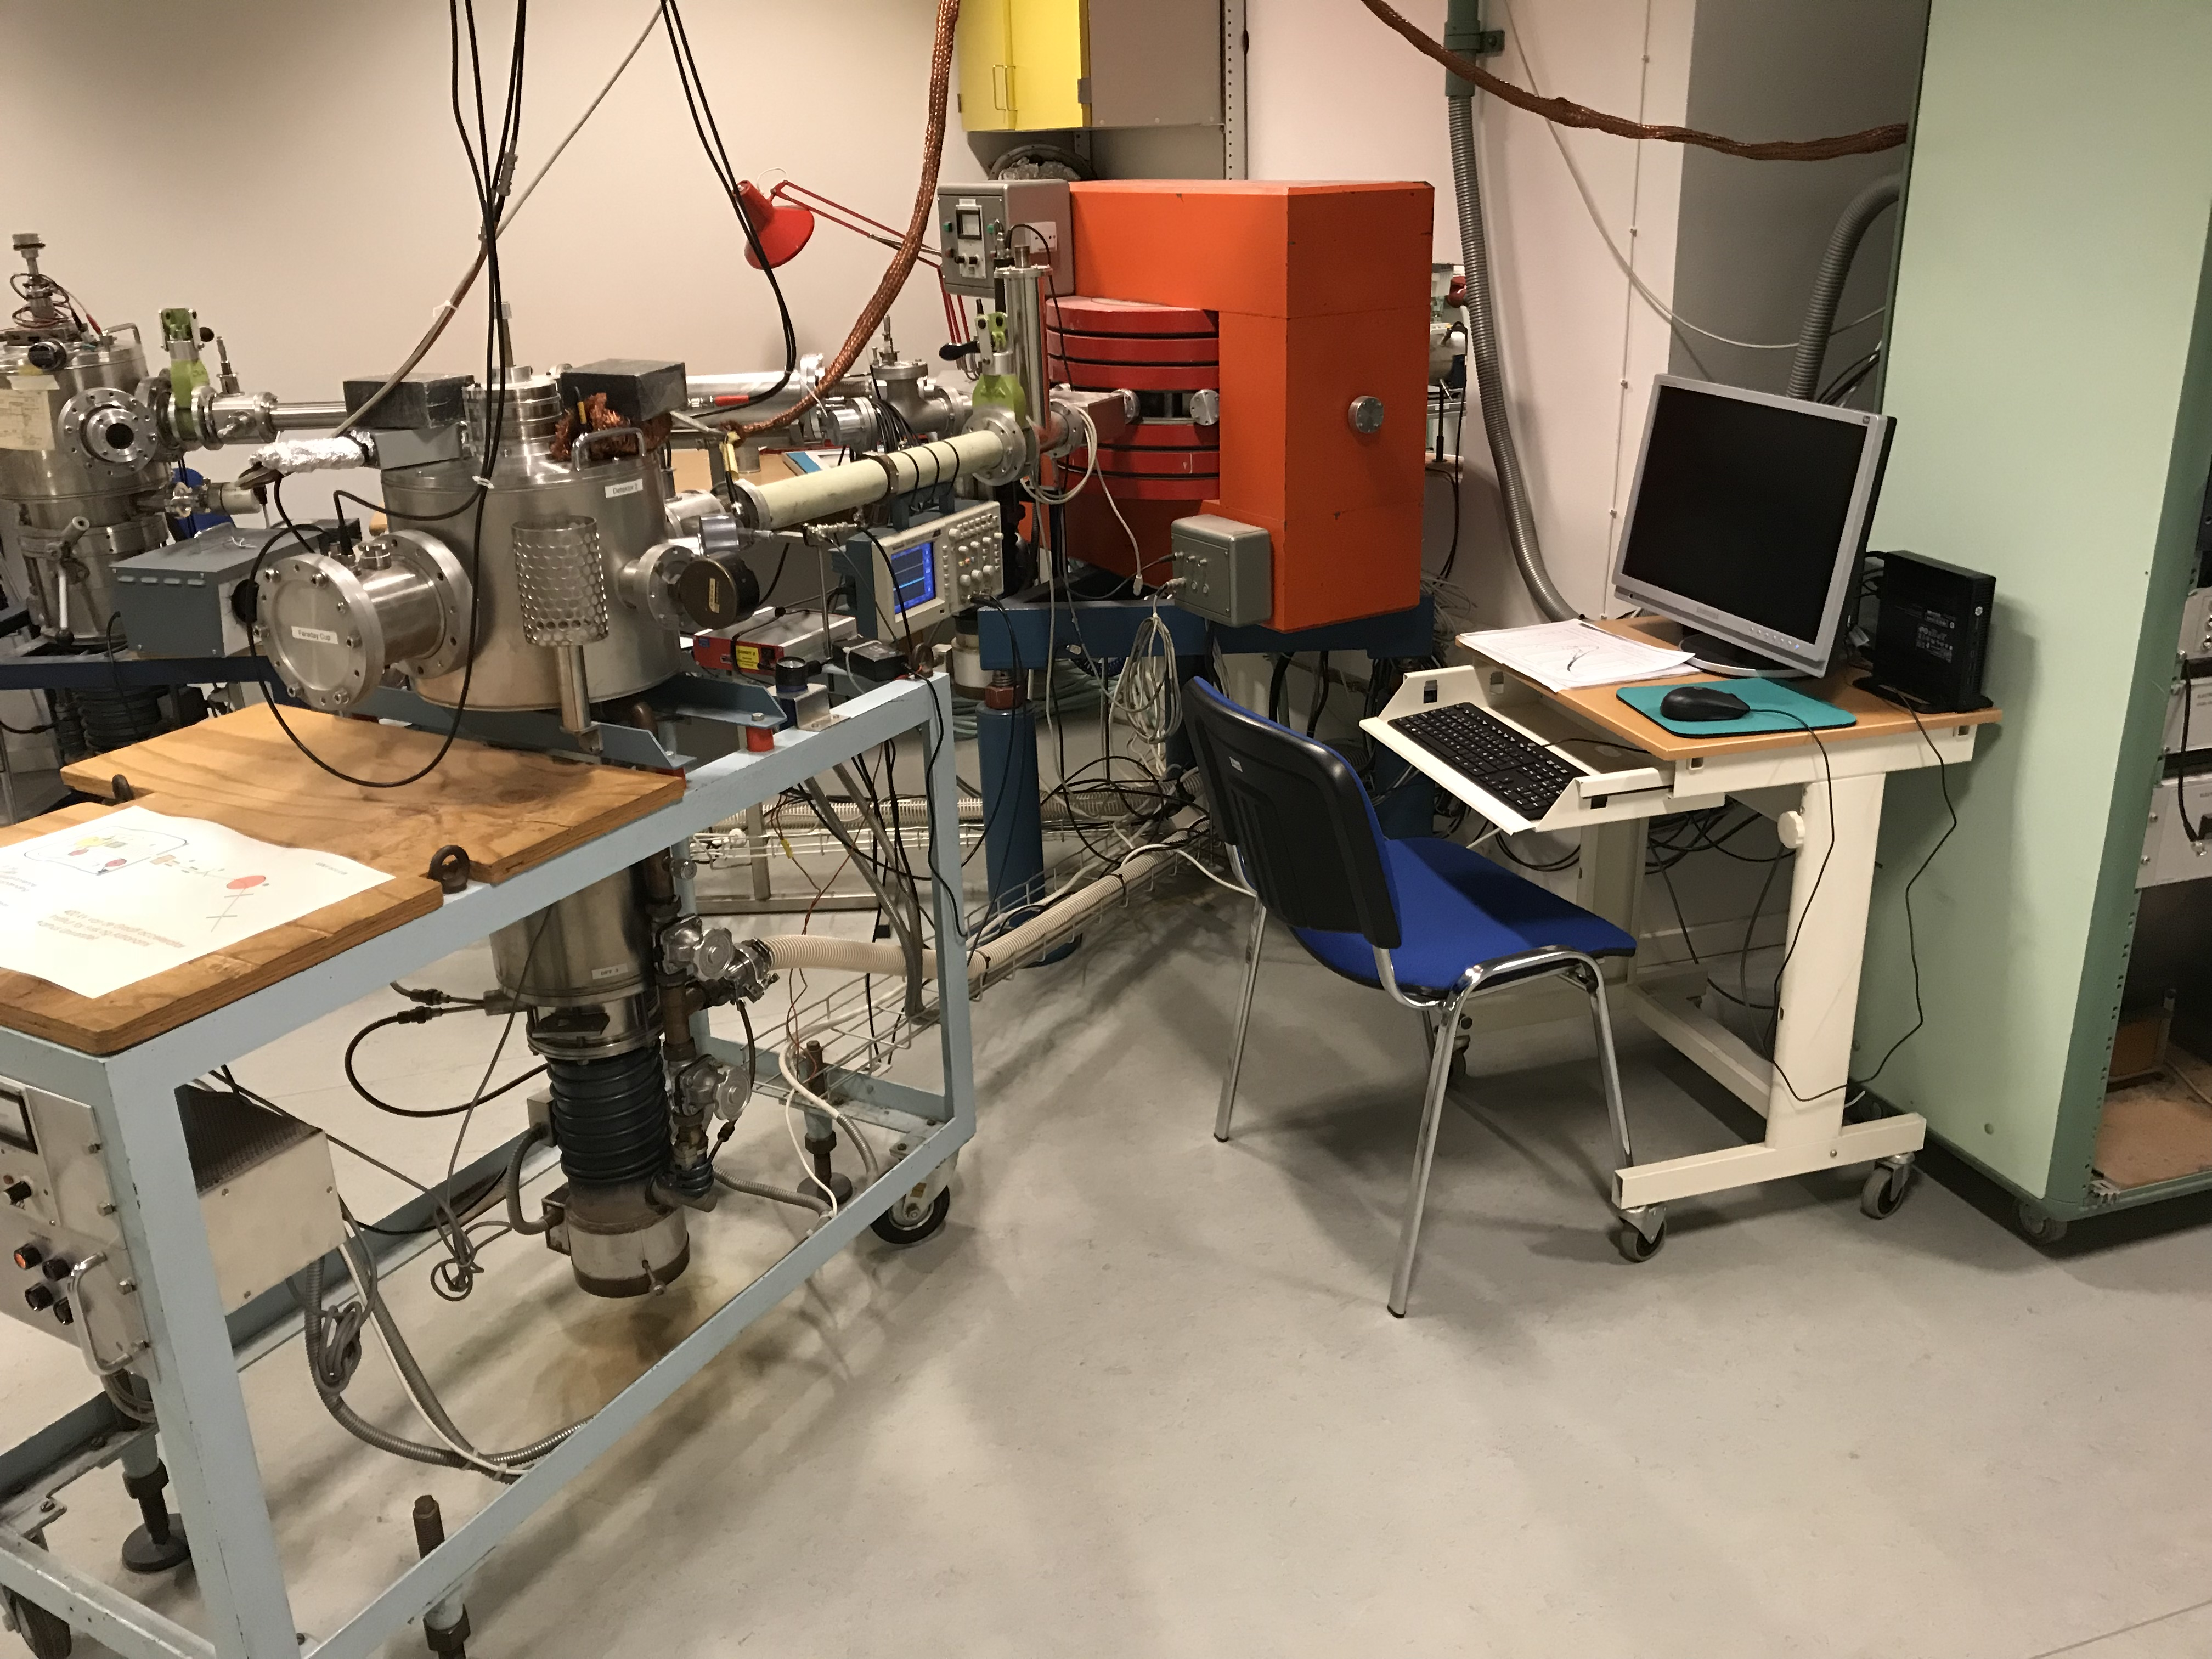
\includegraphics[width=0.99\columnwidth]{setup1}
    \caption{From left to right; Overview of the Faraday cup, Silicium detector, beamline, and electromagnet (red brick).}
    \label{fig_setup1}
\end{figure}
%
\begin{figure}[t]
    \centering
    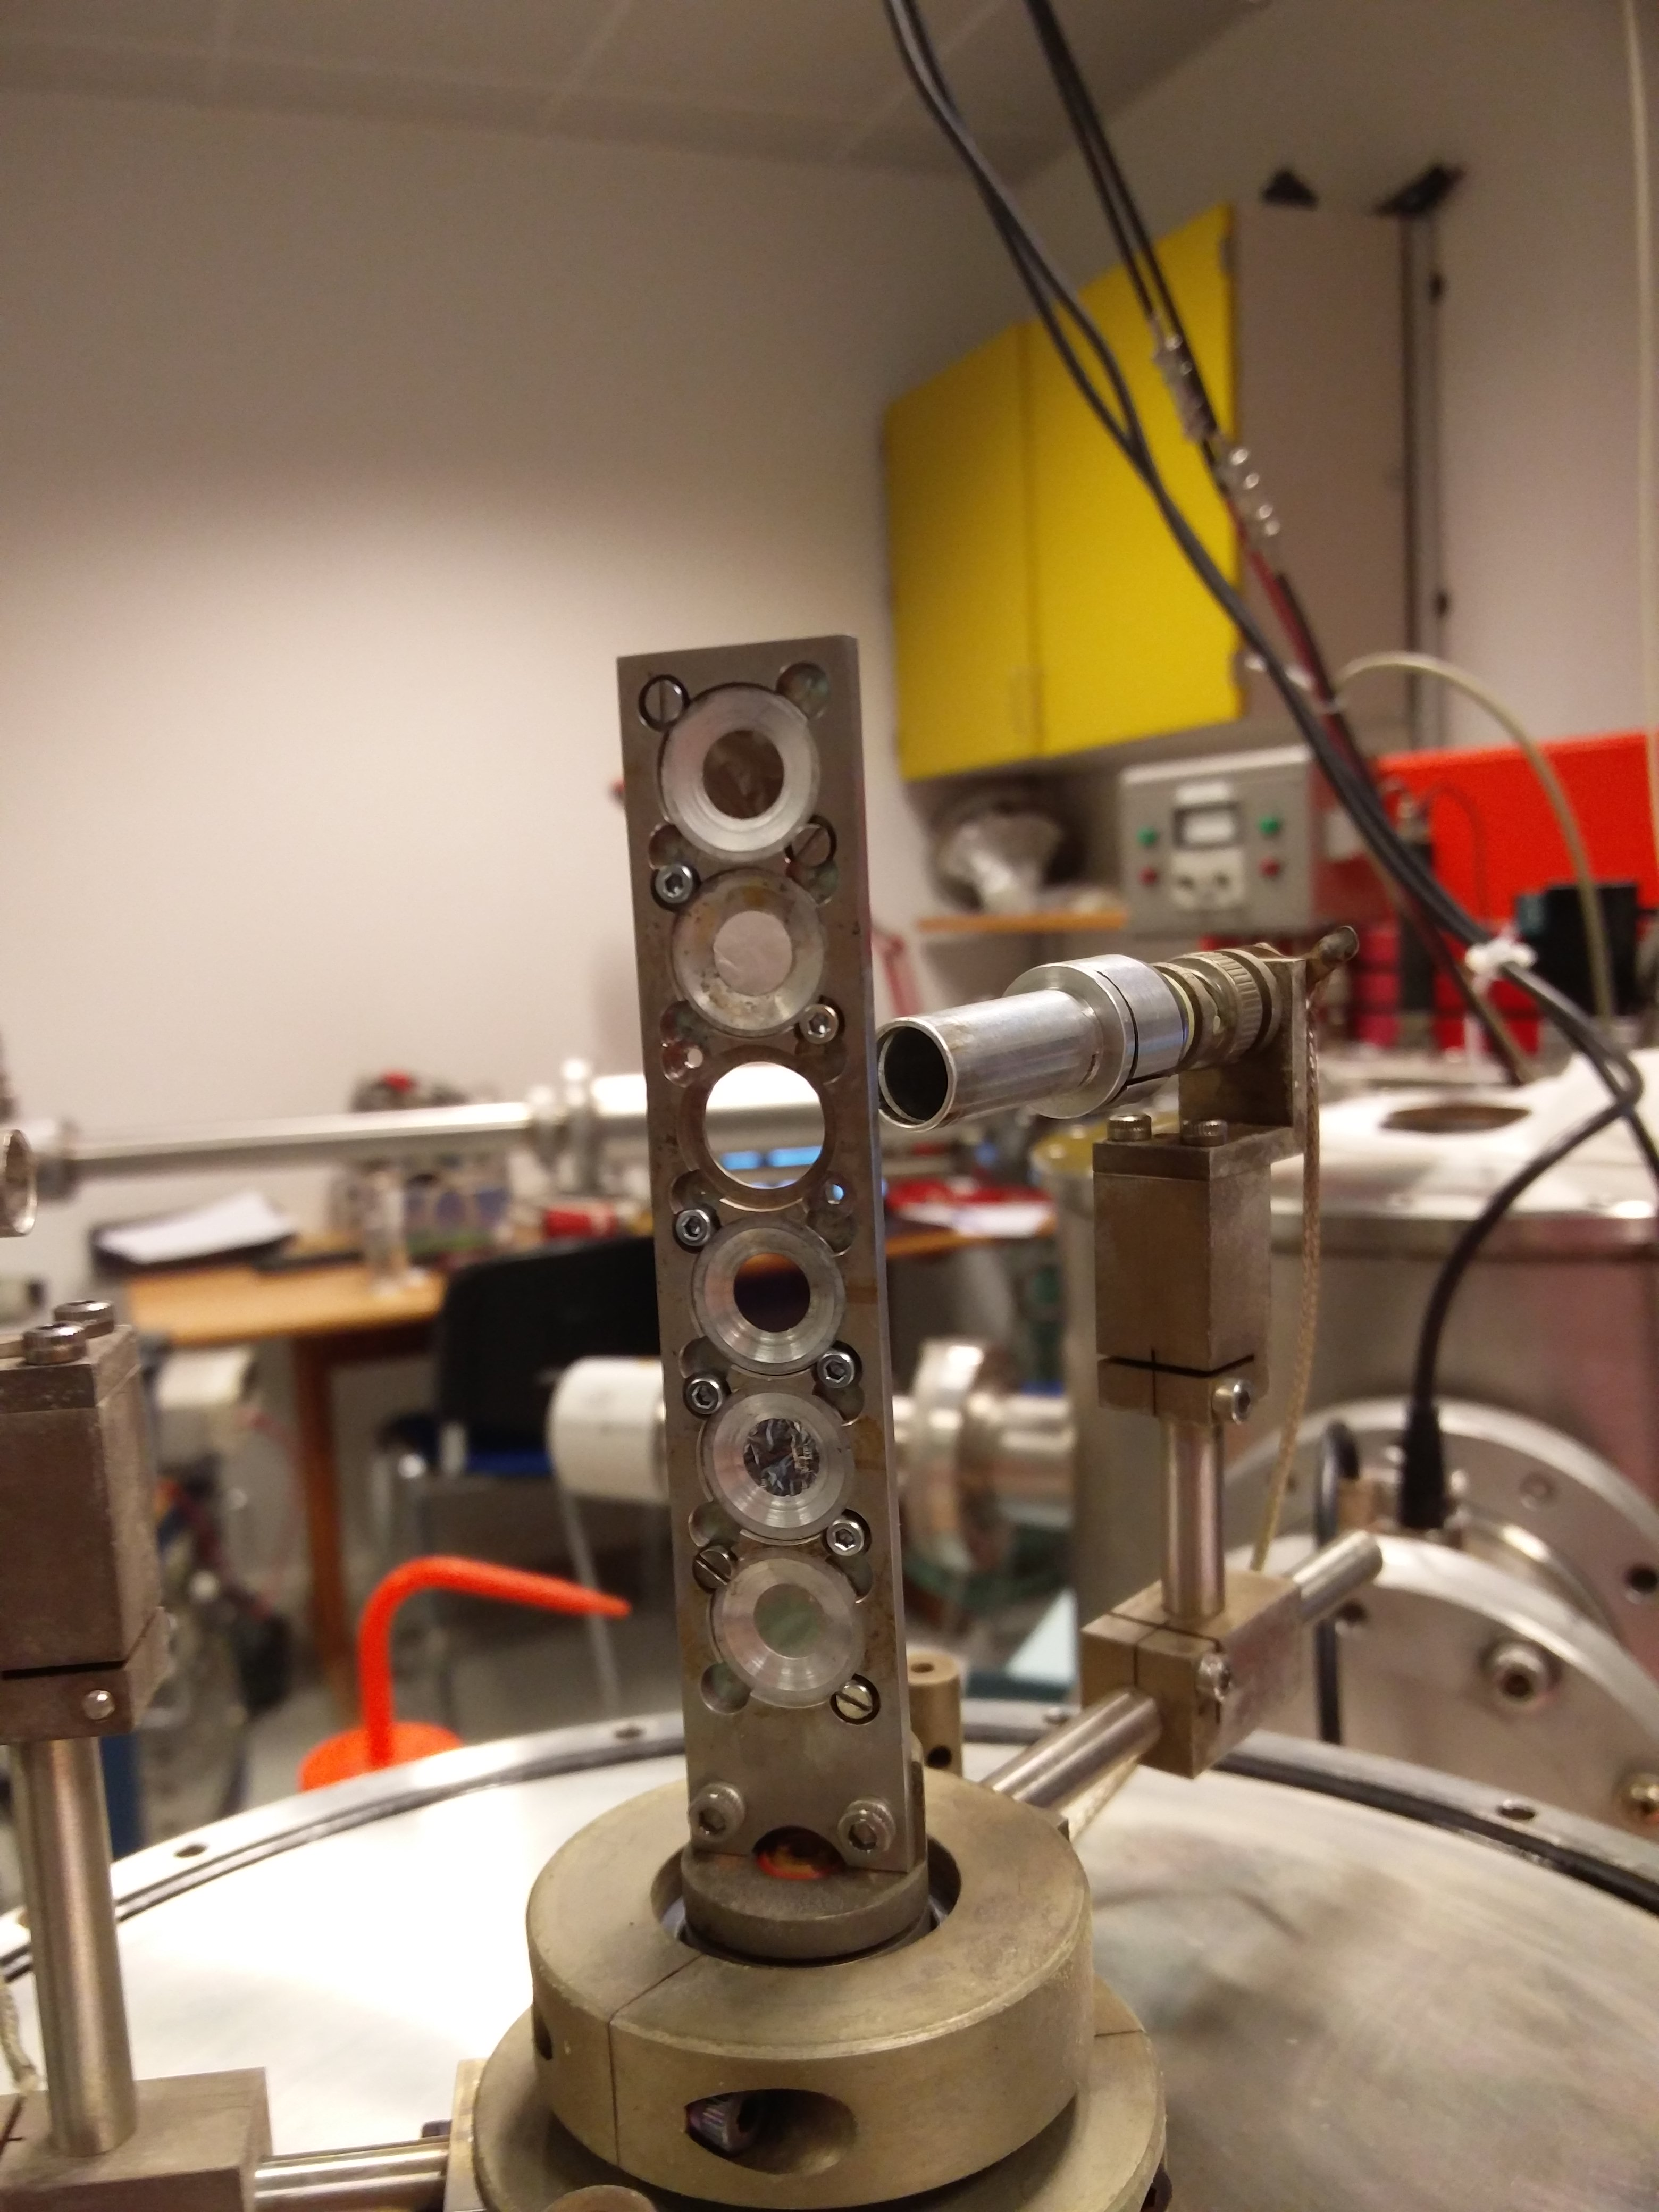
\includegraphics[trim={0cm, 10cm, 0cm, 40cm}, clip, width=0.99\columnwidth]{setup4}
    \caption{The equipment had a failure, so the targets were changed. We were
    lucky to get this picture of both detector and targets.}
    \label{fig_setup4}
\end{figure}
%
Subsequently, the incomming ions were directed towards the thin target foil
\cref{fig_setup4}, and the scattered particles were detected by a Silicon
detector at a variable angle up to $160$ degree relative to the
direct beam. 

The detector was at a constant seperation from the target, $r =
\SI{49\pm1}{\milli\meter}$, and it had a circular area of given diameter
$D=\SI{1.88 \pm 0.01}{\milli\meter}$. Of importance is the solid angle of 
\begin{equation}
d\Omega = \frac{dA}{r^2}
\end{equation}
used in the Rutherford differential cross section later on.

The detector was coupled to a digitizer connected to a computer. During
measurements the digitizer started a clock. When an ion was detected, the
digitizer translated the measured energy into a digital number and sent the
number and the corresponding time stamp to the computer.  The program
Mc2Analyzer was used to handle the data. The digital number is an arbitrary
number called a channel number. It is translatable to the actual energy by a
linear factor plus an offset. In order to convert these channel numbers to
correct energies of the scattered particles a calibration was done.

\subsection{Calibration}
An energy meassurement of the scattered ion gives a digitial output, which we call
a channel number (or bin number). These hold no physical interpretation, but
can be translated to the equivalent energy of the scattered particle. To
convert these channel numbers, a calibration is necesarry. 

Assuming a linear relationship between the energy and the channel number the
energy can be found as
\begin{equation}
    E = \alpha(k - k_|0|), \label{eq_calibration}
\end{equation}
where $k$ is the meassured channel, $k_0$ is the channel number corresponding to
a zero--amplitude input, and $\alpha$ is a conversion parameter.
The parameters in the relation \cref{tab_parameters} is determined by a two
step program.

\begin{table}[b]
\centering
\caption{The values of the parameters, used to convert channel numbers to
energies.}
\begin{tabular}{CC}
\toprule
\multicolumn{2}{c}{Calibration parameters}\\
\midrule
k_|0| & 1.36\pm 0.15 \\
\alpha & 0.800 \pm 0.005 \\
\bottomrule
\end{tabular}

\label{tab_parameters}
\end{table}

\subsubsection{Determing the zero-amplitude constant}
First, by connecting a pulser (variable output voltage), a relation between the
varied energy and the corresponding channel number is obtained. 
We did this for equidistant pulsed energies, and although unimportant for the
time being, we included the threshold pulser amplitude -- the minimal amplitude
for a detected signal.

Data obtained can be plotted as count numbers versus bin numbers. Due to the
central limit theorem \parencite[p. 49]{statistics}, data can be fitted to a
gaussian distribution. This is done for each value of pulsed energy, for which
one gains parameter values for each gaussian within an uncertainty, determined
by the square root of the covariance matrix diagonal \cref{fig_gaussian_fit}.

Each centroid (the mean bin number of the gaussian fit) was then compared as a
function of the pulser amplitude. As expected from \cref{eq_calibration}, this
follows a linear relation \cref{fig_linear_fit}.
The intersection is interpretated as the bin number at zero amplitude ($k_|0|$).

\begin{figure}[t]
\centering
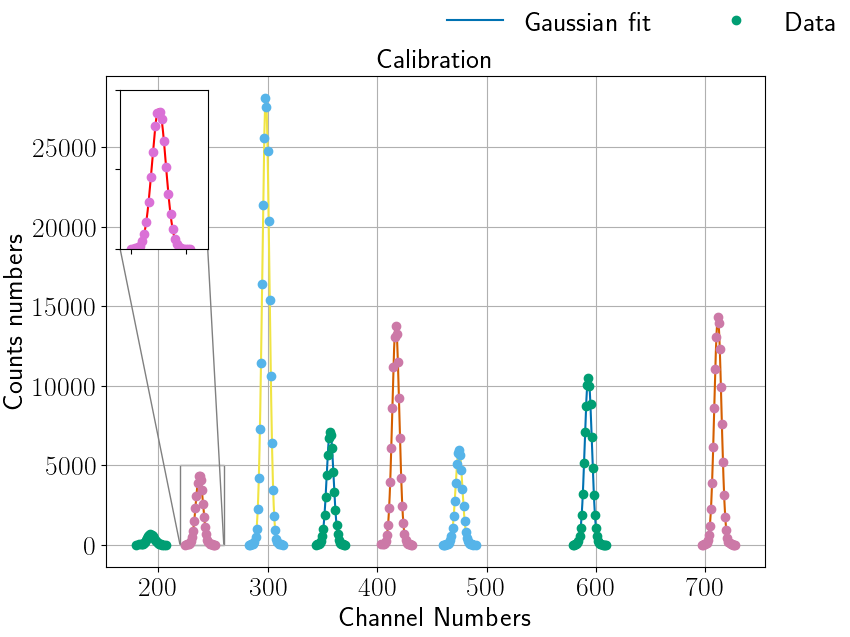
\includegraphics[width=0.99\columnwidth]{gaussian_fit}
\caption{Gaussian fits for all data meassured pulser-amplitude-signals. This was used to estimate the mean
bin number (centroid), and the uncertainty of the parameters used in the
energy-calibration.}
\label{fig_gaussian_fit}
\end{figure}

\begin{figure}[t]
\centering
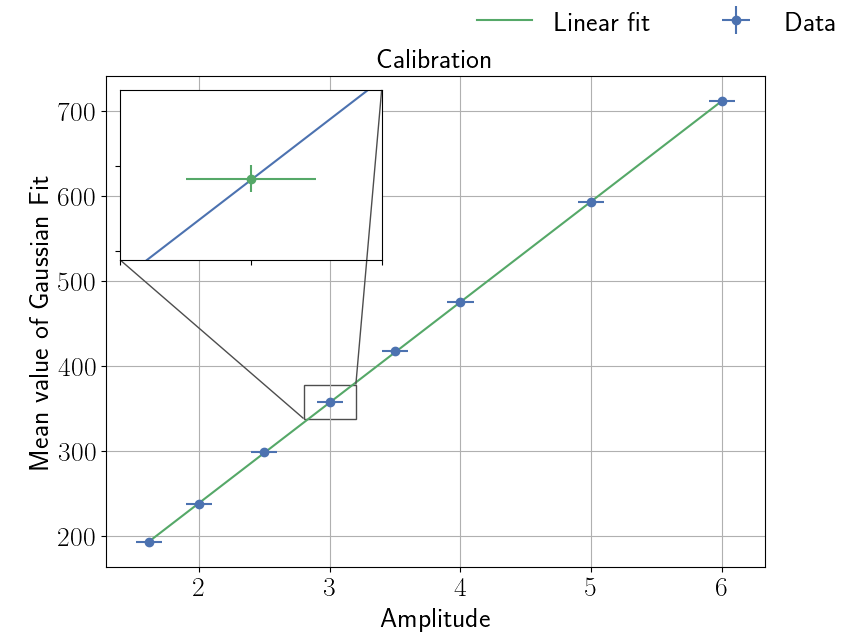
\includegraphics[width=0.99\columnwidth]{k0_plotting}
\caption{Linear fit of the mean values as a function of amplitude. This was
used to determine the zero-amplitude constant $k_|0|$.}
\label{fig_linear_fit}
\end{figure}

 
\subsubsection{Determining alpha}
As described in the previous section, the magnetic field strength of the
electromagnet can be adjusted to deflect either $\mathrm{H^+}$ or
$\mathrm{{H_2}^+}$ into the beamline. For each of these a data point of energy
related to channel number can be found at a given angle.

The energy of the scattered particles, $E_|f|$, can be found by energy and
momentum conservation considerations for elastic scattering in two dimensions.
One is lead to the relation;
\begin{equation}
E_|f| = \left( \frac{m_|p| \cos\theta + \sqrt{{m_|t|}^2 - {m_|p|}^2
\sin^2\theta}}{m_|p|+m_|t|} \right)^2 E_|i|,
\label{eq_5}
\end{equation}
where $E_|i|$ is the energy of the incident beam particles, $m_|p|$ and $m_|t|$ are
the masses of the incident and the target particles, respectively. 
$\theta$ is the angle between the direct outgoing non-scattered beam and the
scattered particles - also called the scattering angle.

Unfortunately, this only gives two data points one from $\mathrm{H^+}$ and
another from $\mathrm{{H_2}^+}$. Nonetheless, the incline from the linear fit
to these data points is still useful. However, a work around solution
for this specific problem exists. By using a target of two layers; gold and carbon
respectively, we have multiple centroids; one for $\mathrm{H_2^+}$ and the gold
layer, another two for $\mathrm{H^+}$
scattering off both gold and carbon \cref{fig_gaussian_fit2}. Thus the linear fit
\cref{fig_linear_fit2} has a third point.

One should be aware of the difference between the two linear fits. First we
fitted for two parameters, both incline and intersection, and obtained the
value of the zero-amplitude bin value \cref{fig_linear_fit}. Afterwards, we fitted for a single
parameter, the incline, and used the value of $k_|0|$ \cref{fig_linear_fit2}.

\begin{figure}[t]
\centering
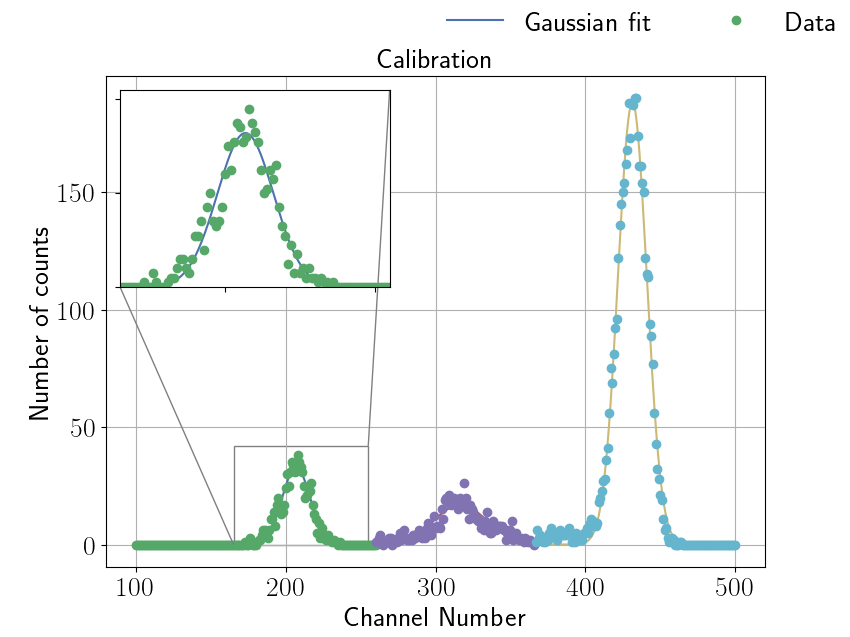
\includegraphics[width=0.99\columnwidth]{gaussian_fit2}
\caption{From left to right we see $\mathrm{H_|2|^{+}}$ scattering off the gold layer
and $\mathrm{H^+}$ scattering off the carbon and gold layer respectively.}
\label{fig_gaussian_fit2}
\end{figure}

\begin{figure}[t]
\centering
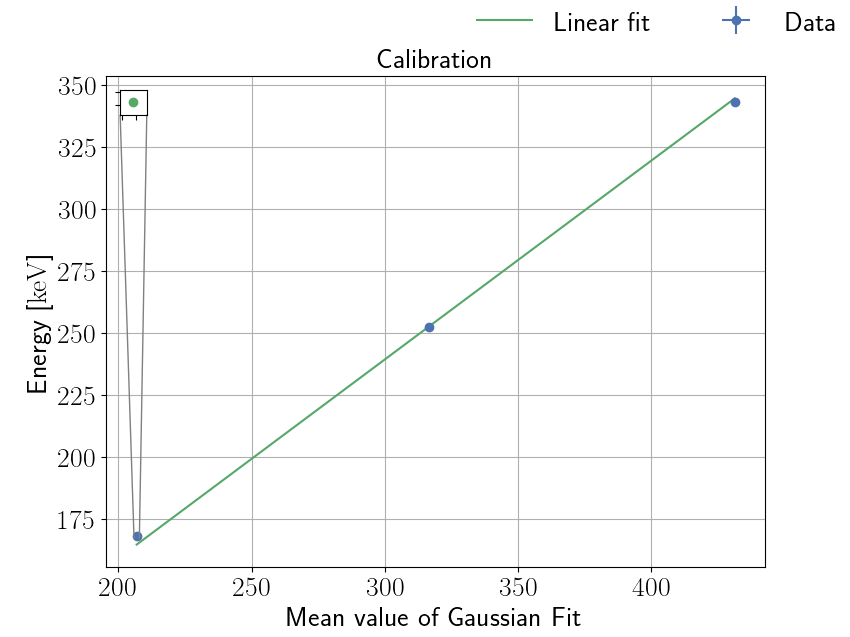
\includegraphics[width=0.99\columnwidth]{alpha_plotting}
\caption{A linear fit of three points.}
\label{fig_linear_fit2}
\end{figure}

%\subsection{Targets}
%\fxnote{FIX}
%The targets of interest in this experiment was a thin gold coated carbon plate. The gold coating was about one tenth of the carbon thickness. The thickness of the carbon plate have previously been determined as $\SI{250}{\angstrom}$, and the thickness of the gold coating as $\SI{25}{\angstrom}$.\footnotemark \footnotetext{The estimated thickness of each target available have been determined by the previous users of the experimental setup and written down on the whiteboard next to the setup.} 
%The target was placed in holder, which contains several other targets. The height of the holder was fixed, though it was not investigated whether the marked height was optimal with respect to the beam position.\\
%
%When measuring proton scattering at different angles, the blind angles of the
%target holder may cause a problem. In order to avoid the targets "blind-spots",
%the target was turned at an angle following the detector while still avoiding
%the incoming proton beam to hit a blind angle. The blind angles of the holder
%are around $\pm SI{30}{\degree}$ in each side of the target holder, see figure .  



%\subsection{Scattering on atomic nuclei}
%The aim of this experiment was to use a particle accelerator to test certain dependencies of Rutherford scattering. Numerically, the Rutherford scattering differential cross section per target atom for any target atom is
%\begin{equation}
%\frac{d\sigma}{d\Omega} = 1.296 \left( \frac{Z_1 Z_2}{E_\infty [MeV] \, \sin^2 \left(\frac{\theta}{2} \right) }\right)^2\left[\frac{mb}{sr}\right],
%\end{equation}
%where $\theta$ is the scattering angle, $Z_1$  is the atomic number of the incident particles, $Z_2$ is the atomic number of the target nuclei, and $E_{\infty}$ is their kinetic energy HUSK CITE!%cite 
%. 
%In order to test these dependencies a relation between the cross section and the count rate (number of scattered particles per time) is found as
%\begin{equation}
%dN = N \, n_{\text{tar}} \, dx \,d\Omega \, \frac{d\sigma(\theta,\phi)}{d\Omega},
%\end{equation}
%where $N$ is the number of incoming particles per time, $n_\text{tar}$ is the particle density of the target, $dx$ is the thickness of the target, and $d\Omega$ is the solid angle of the detector.
%
\clearpage
\subsection{Procedure}\label{sec_procedure}
For a complete description of the experimental setup, we have provided this
short review of the startup procedure. This can be omitted, but found valueable
for the course examination.

First thing, the Van-de-Graaff. To accelerate the beam of incomming particles,
one has to generate a high potential. Turning on the belt, one hears the
mechanical rhumming. This will generate a potential difference as described
further in \cite[p. 565]{krane}.
\begin{figure}[h!]
\centering
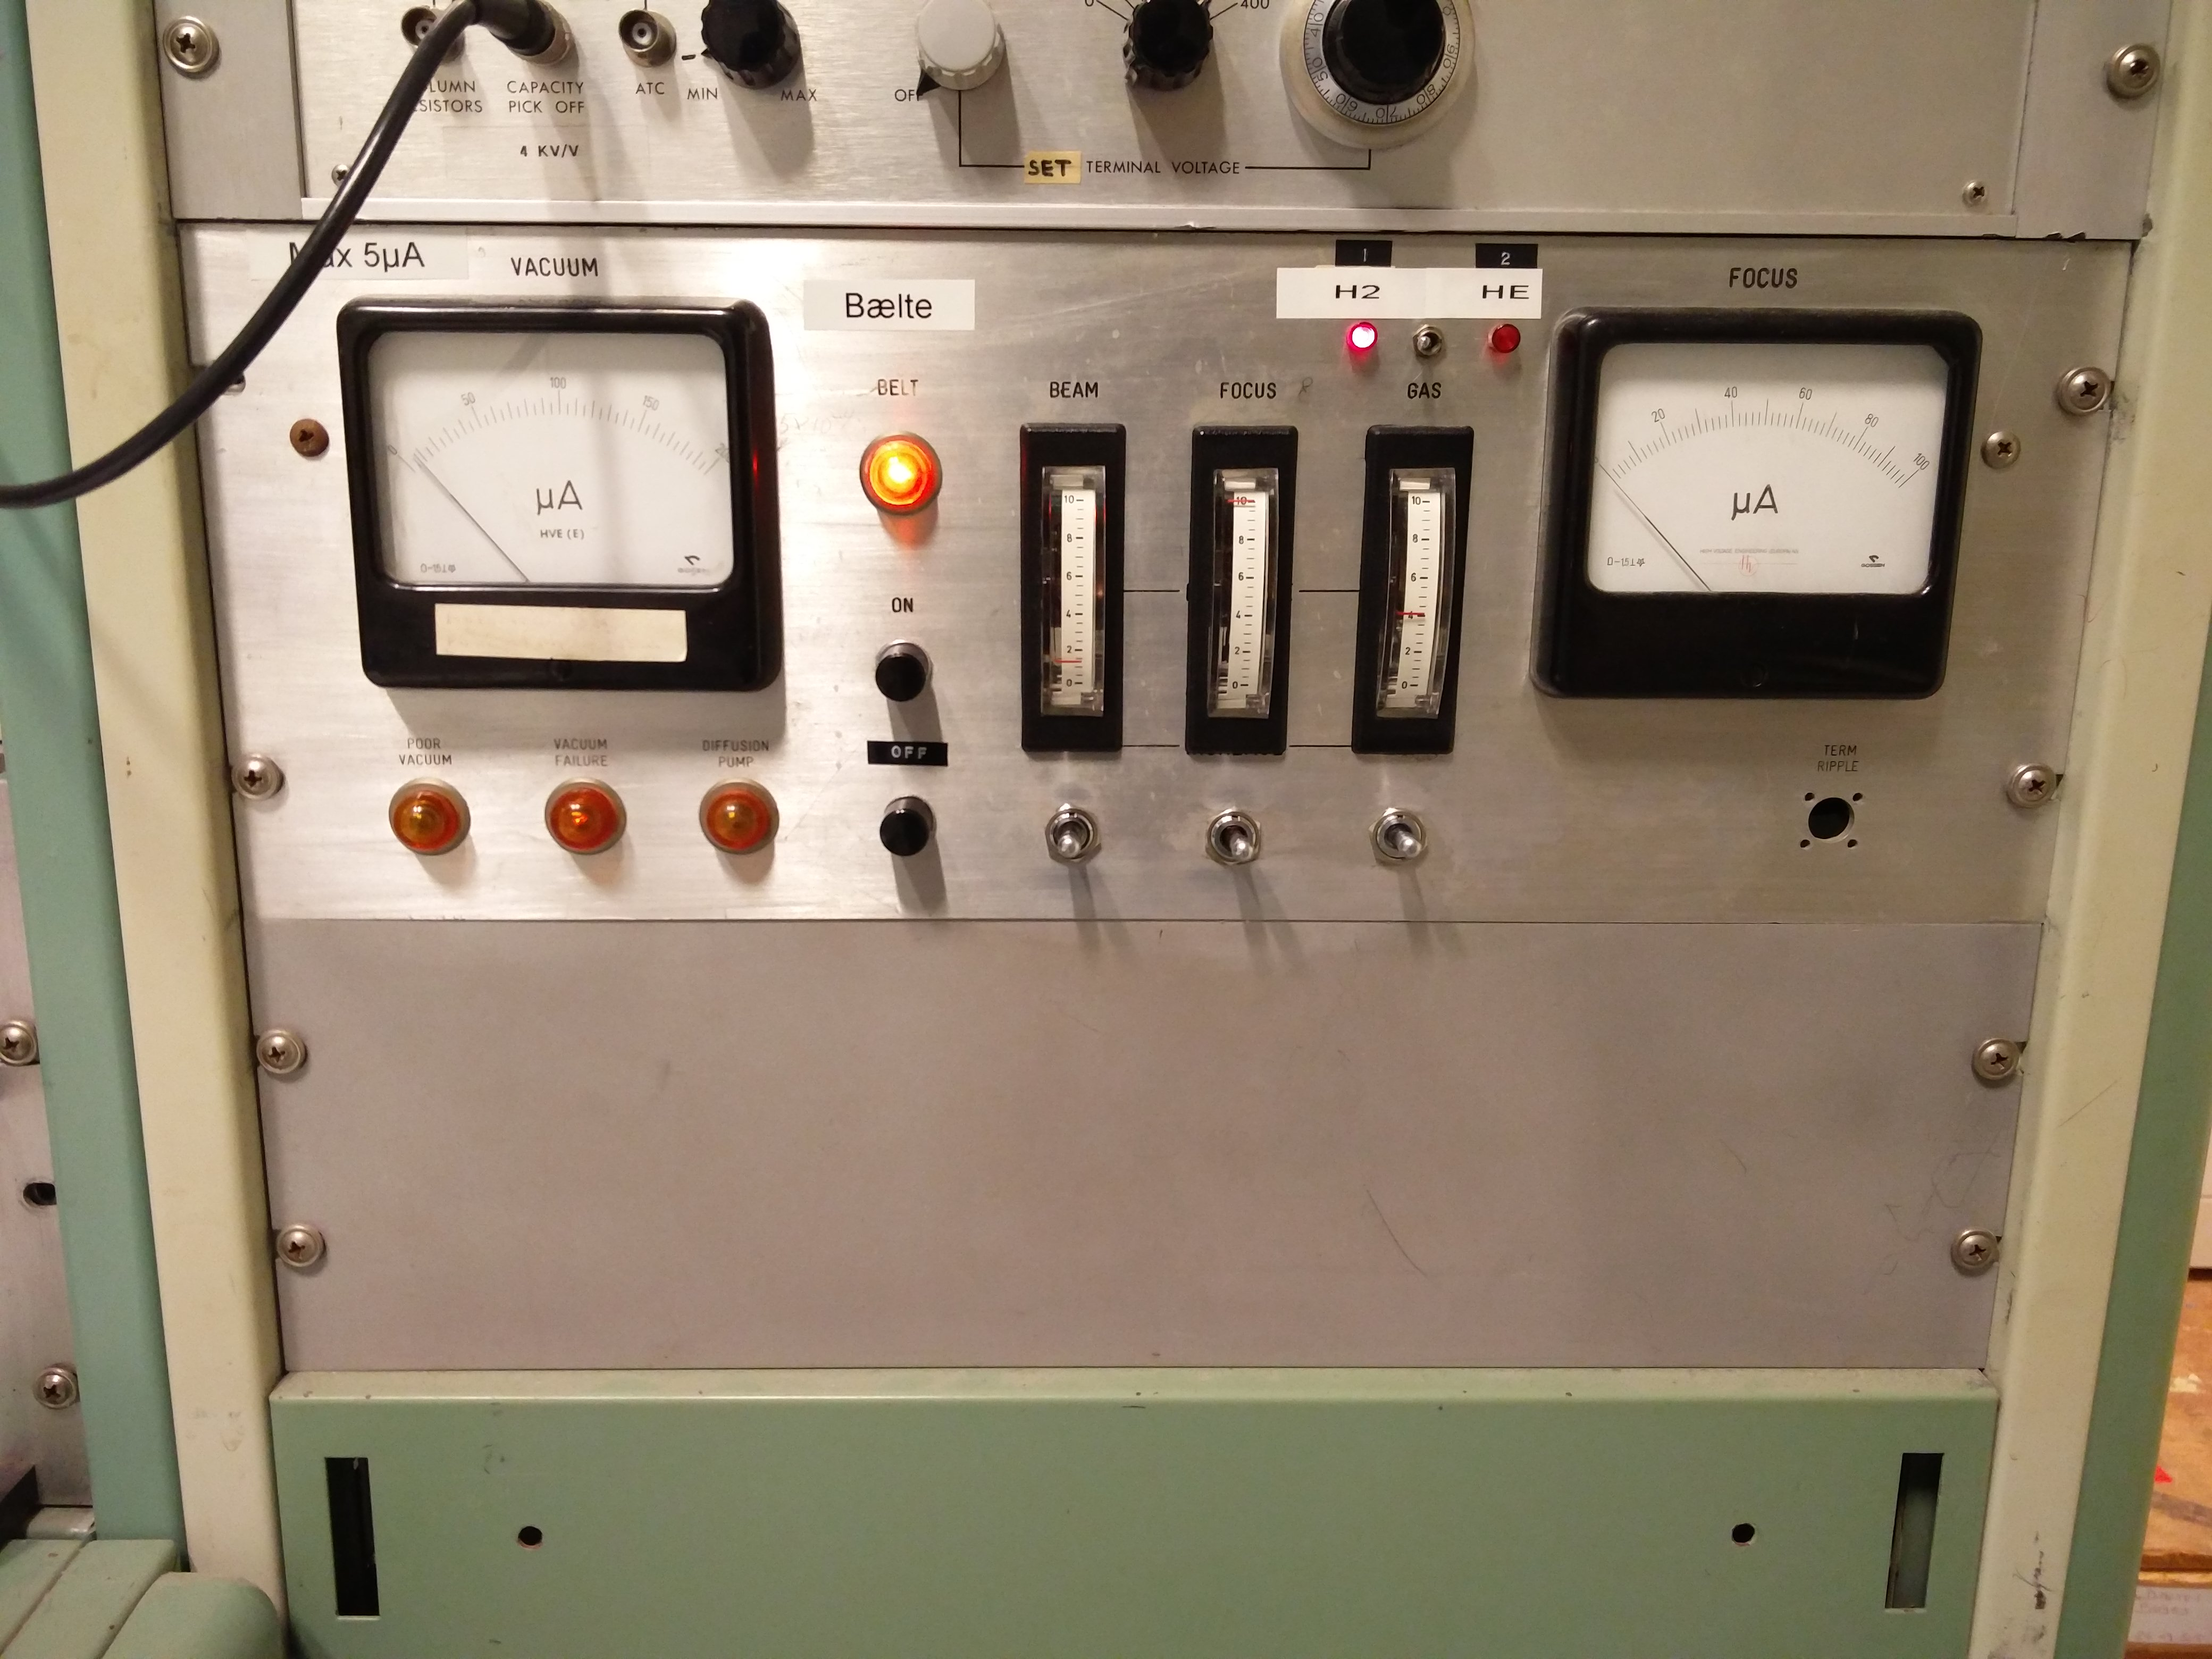
\includegraphics[trim={0, 45cm, 0, 15cm}, clip, width=0.9\columnwidth]{process1}
\caption{The belt is turned on.}
\label{fig_process1}
\end{figure}

Now adjust the terminal voltage patiently towards the desired energy. Our lab
instructor advised us to wait for each step, before going to the next.
\begin{figure}[h!]
\centering
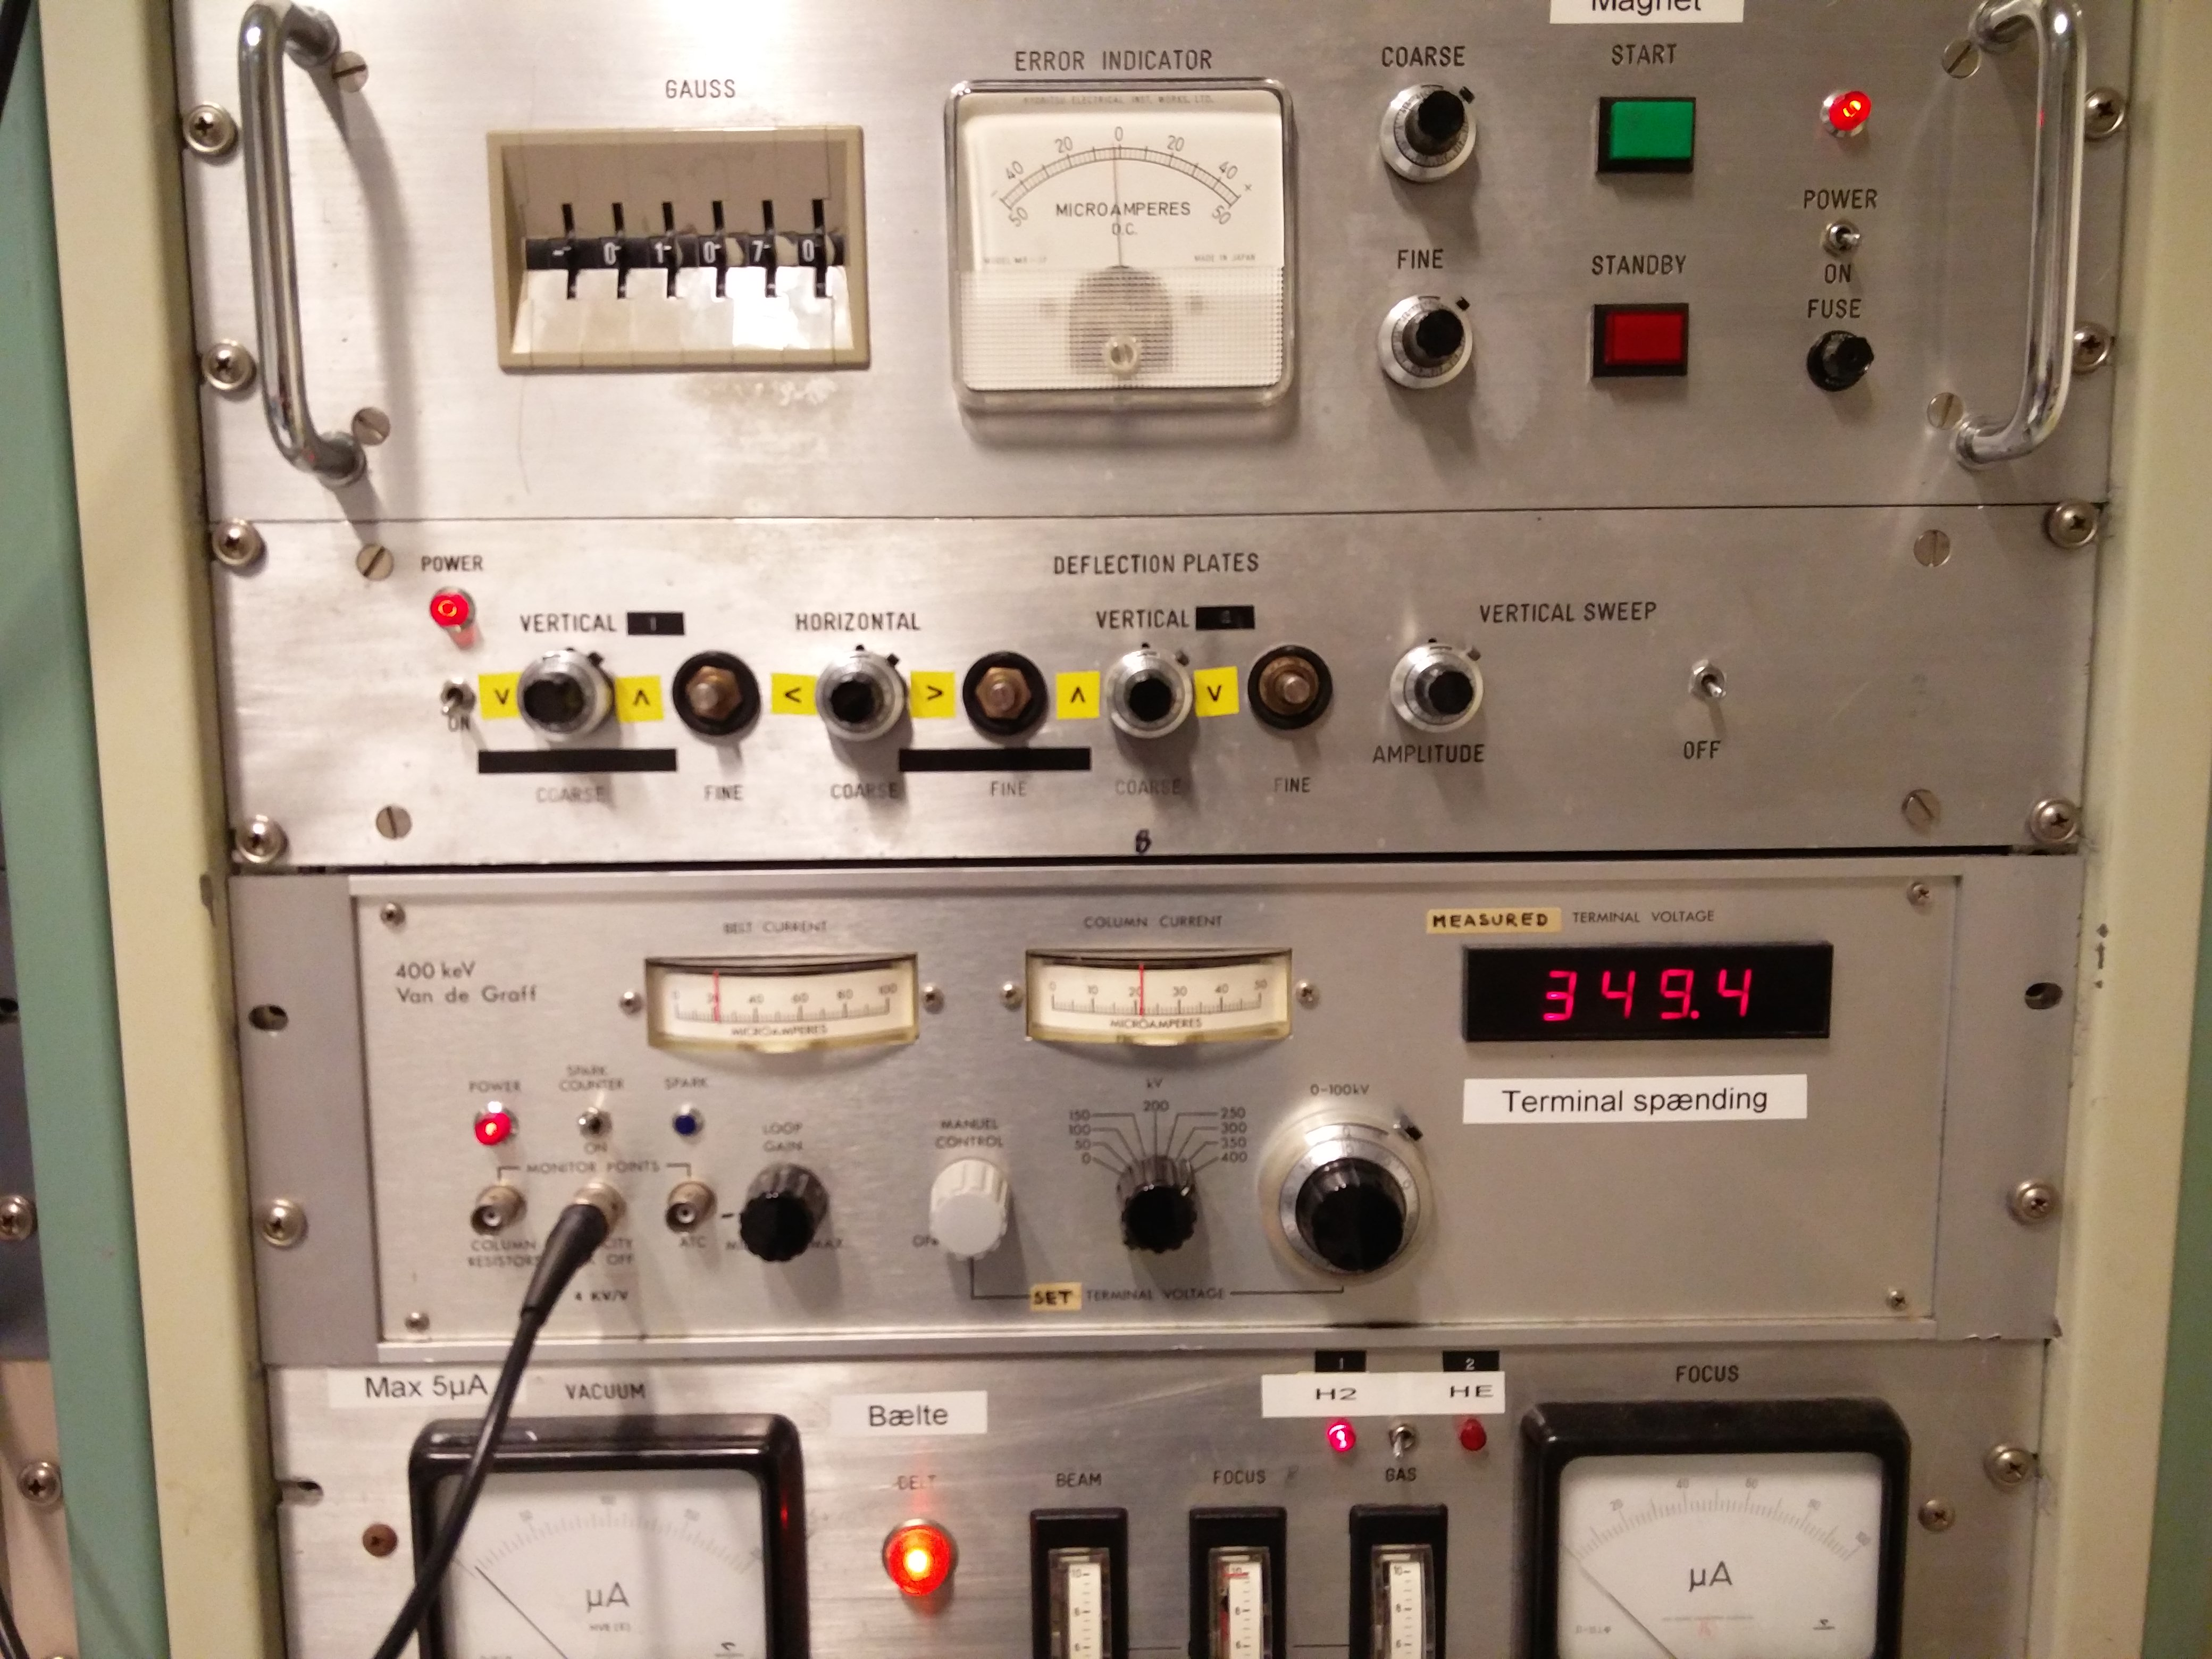
\includegraphics[trim={0, 20cm, 0, 55cm}, clip, width=0.9\columnwidth]{process2}
\caption{Terminal voltage is adjusted to $\SI{350}{\kilo\electronvolt}$.}
\label{fig_process2}
\end{figure}

Turn on the electromagnet. One can dial in the calculated magnetic field
strength. This will do absolutely nothing to the experimental setup, but to
translate the origin of the scale. To change the magnetic field strength, one
has to change the current throught the electromagnet.
\begin{figure}[h!]
\centering
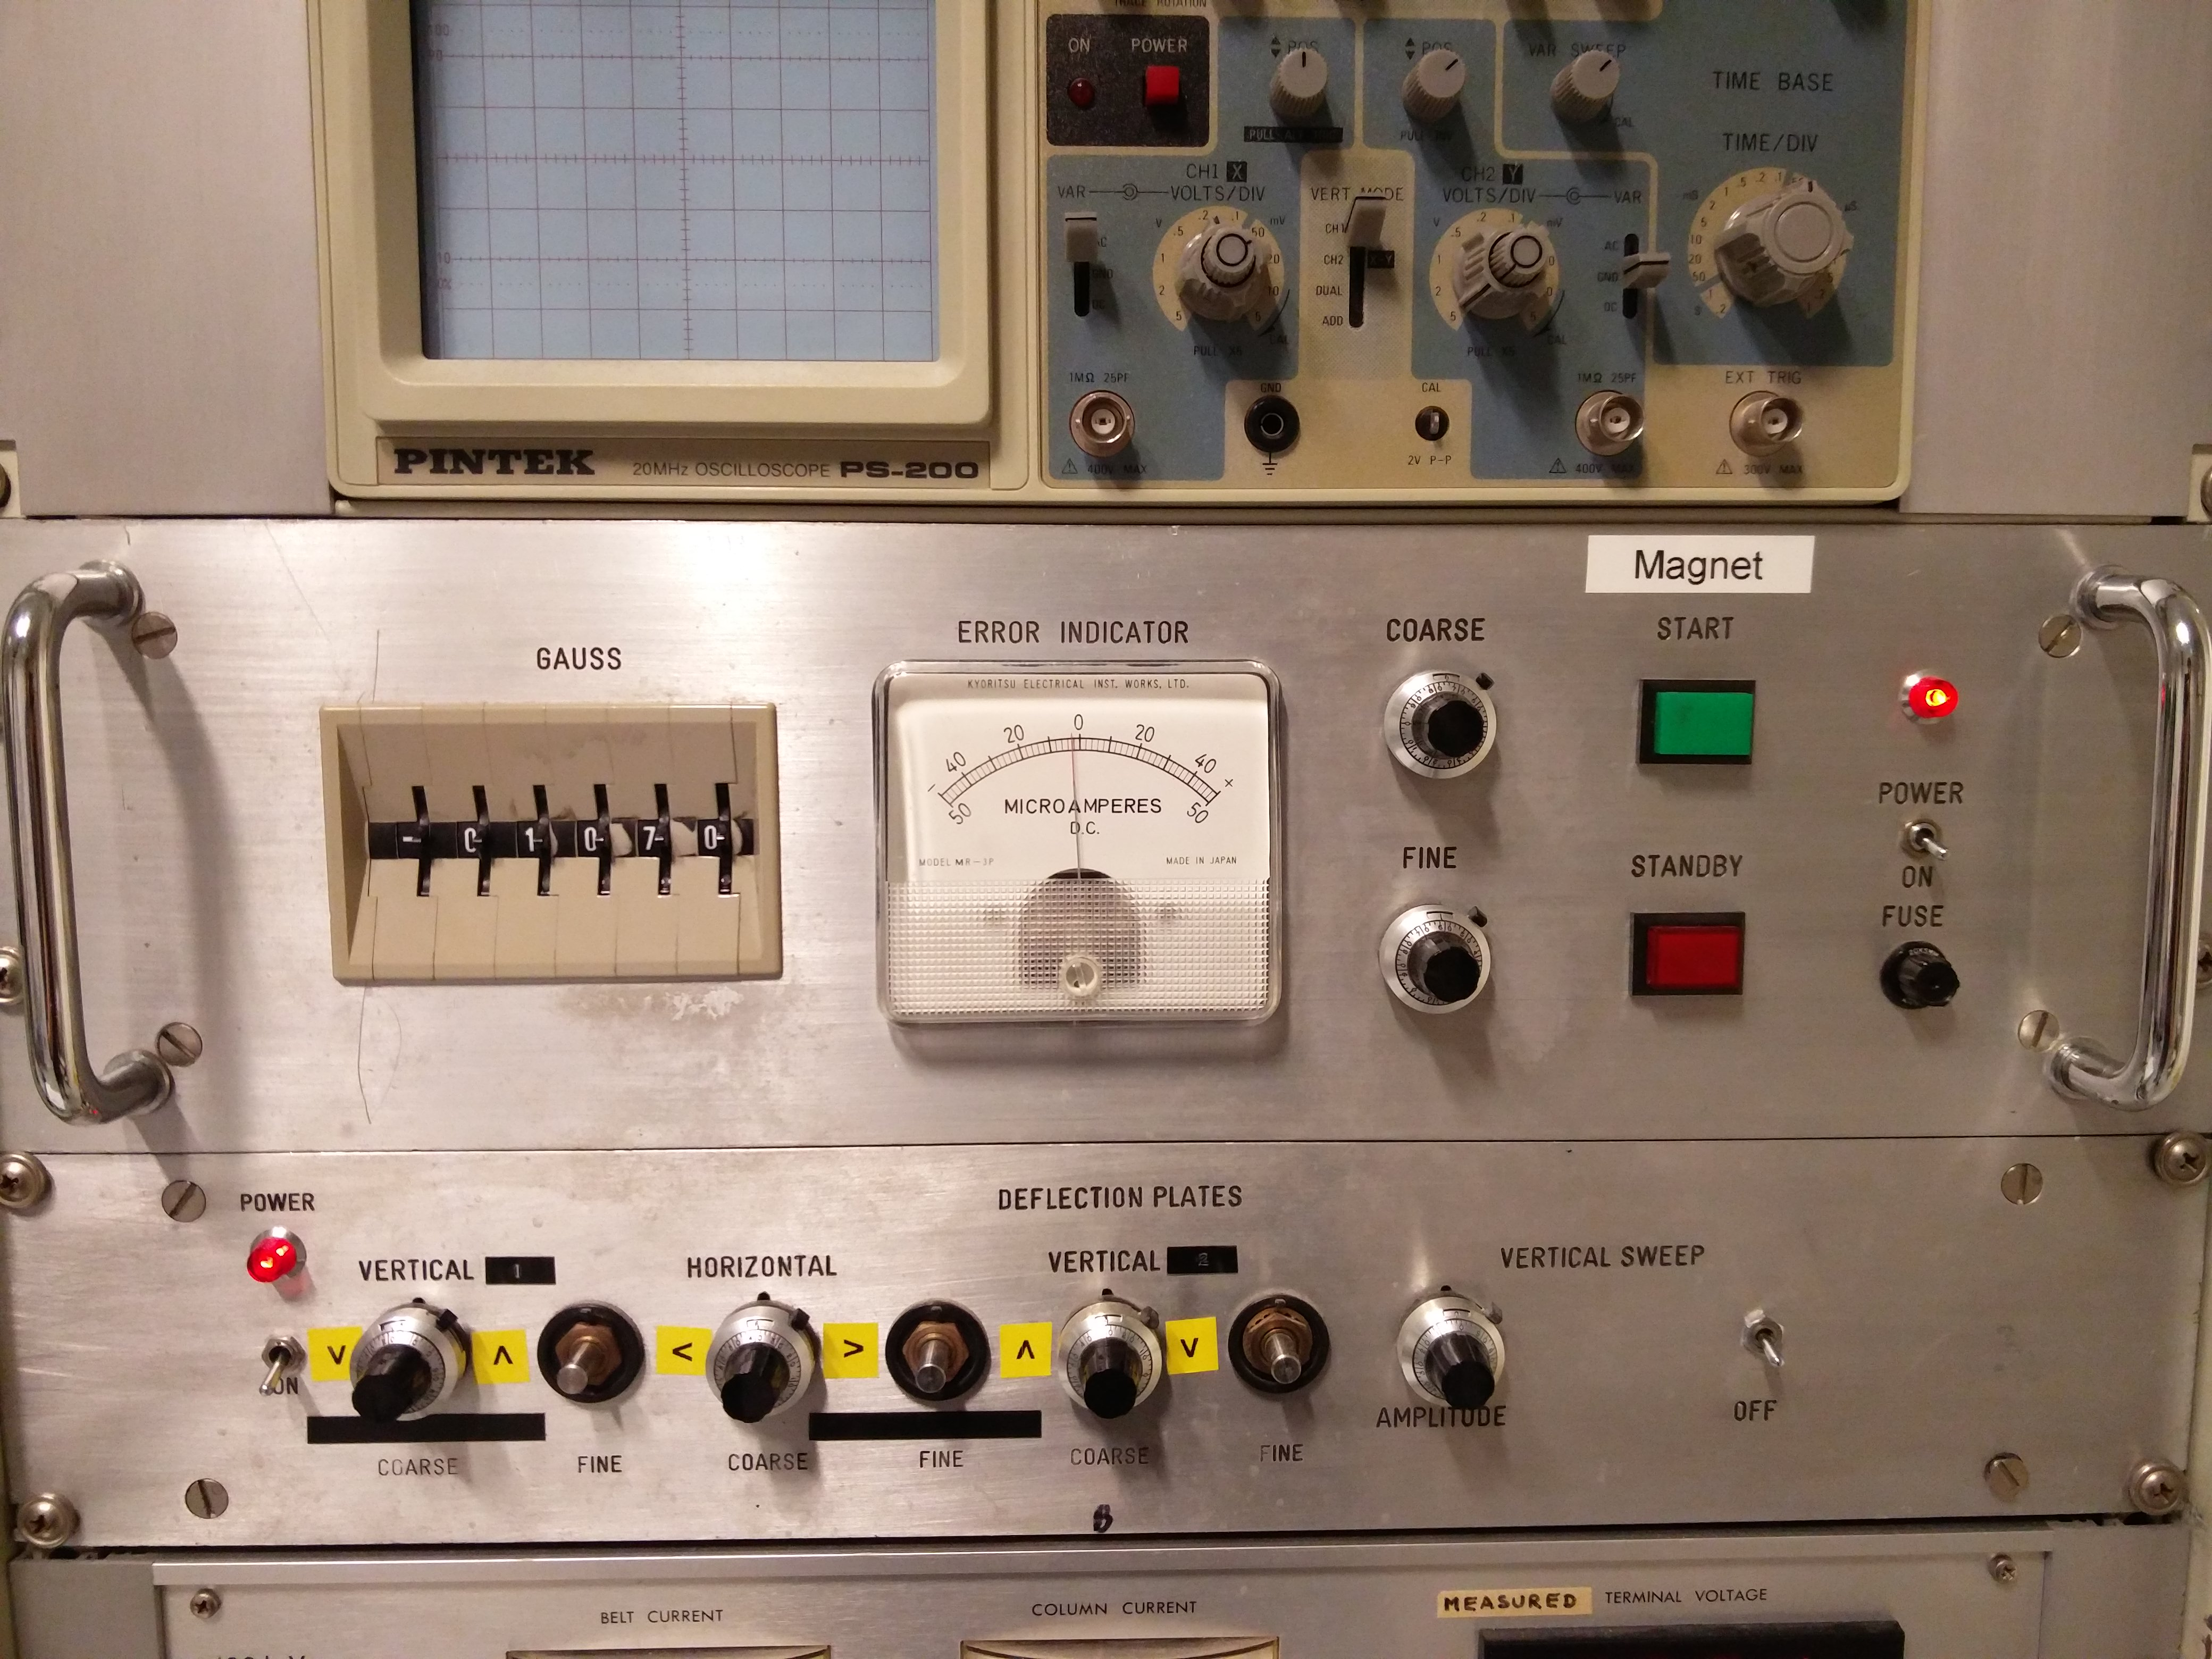
\includegraphics[trim={0, 30cm, 0, 30cm}, clip, width=0.9\columnwidth]{process3}
\caption{Dashboard for the electromagnet.}
\label{fig_process3}
\end{figure}

Now open the vacuum valve, so the incomming ions can be detected.
If the Faraday cup (detector for $0$ degree scattering) is connected to an Ampere
meter, one can look for received current of charged particles. This should be
maximized, by a variational principle about the calculated magnetic field,
using the fine grid for adjustments.

\begin{figure}[h!]
\centering
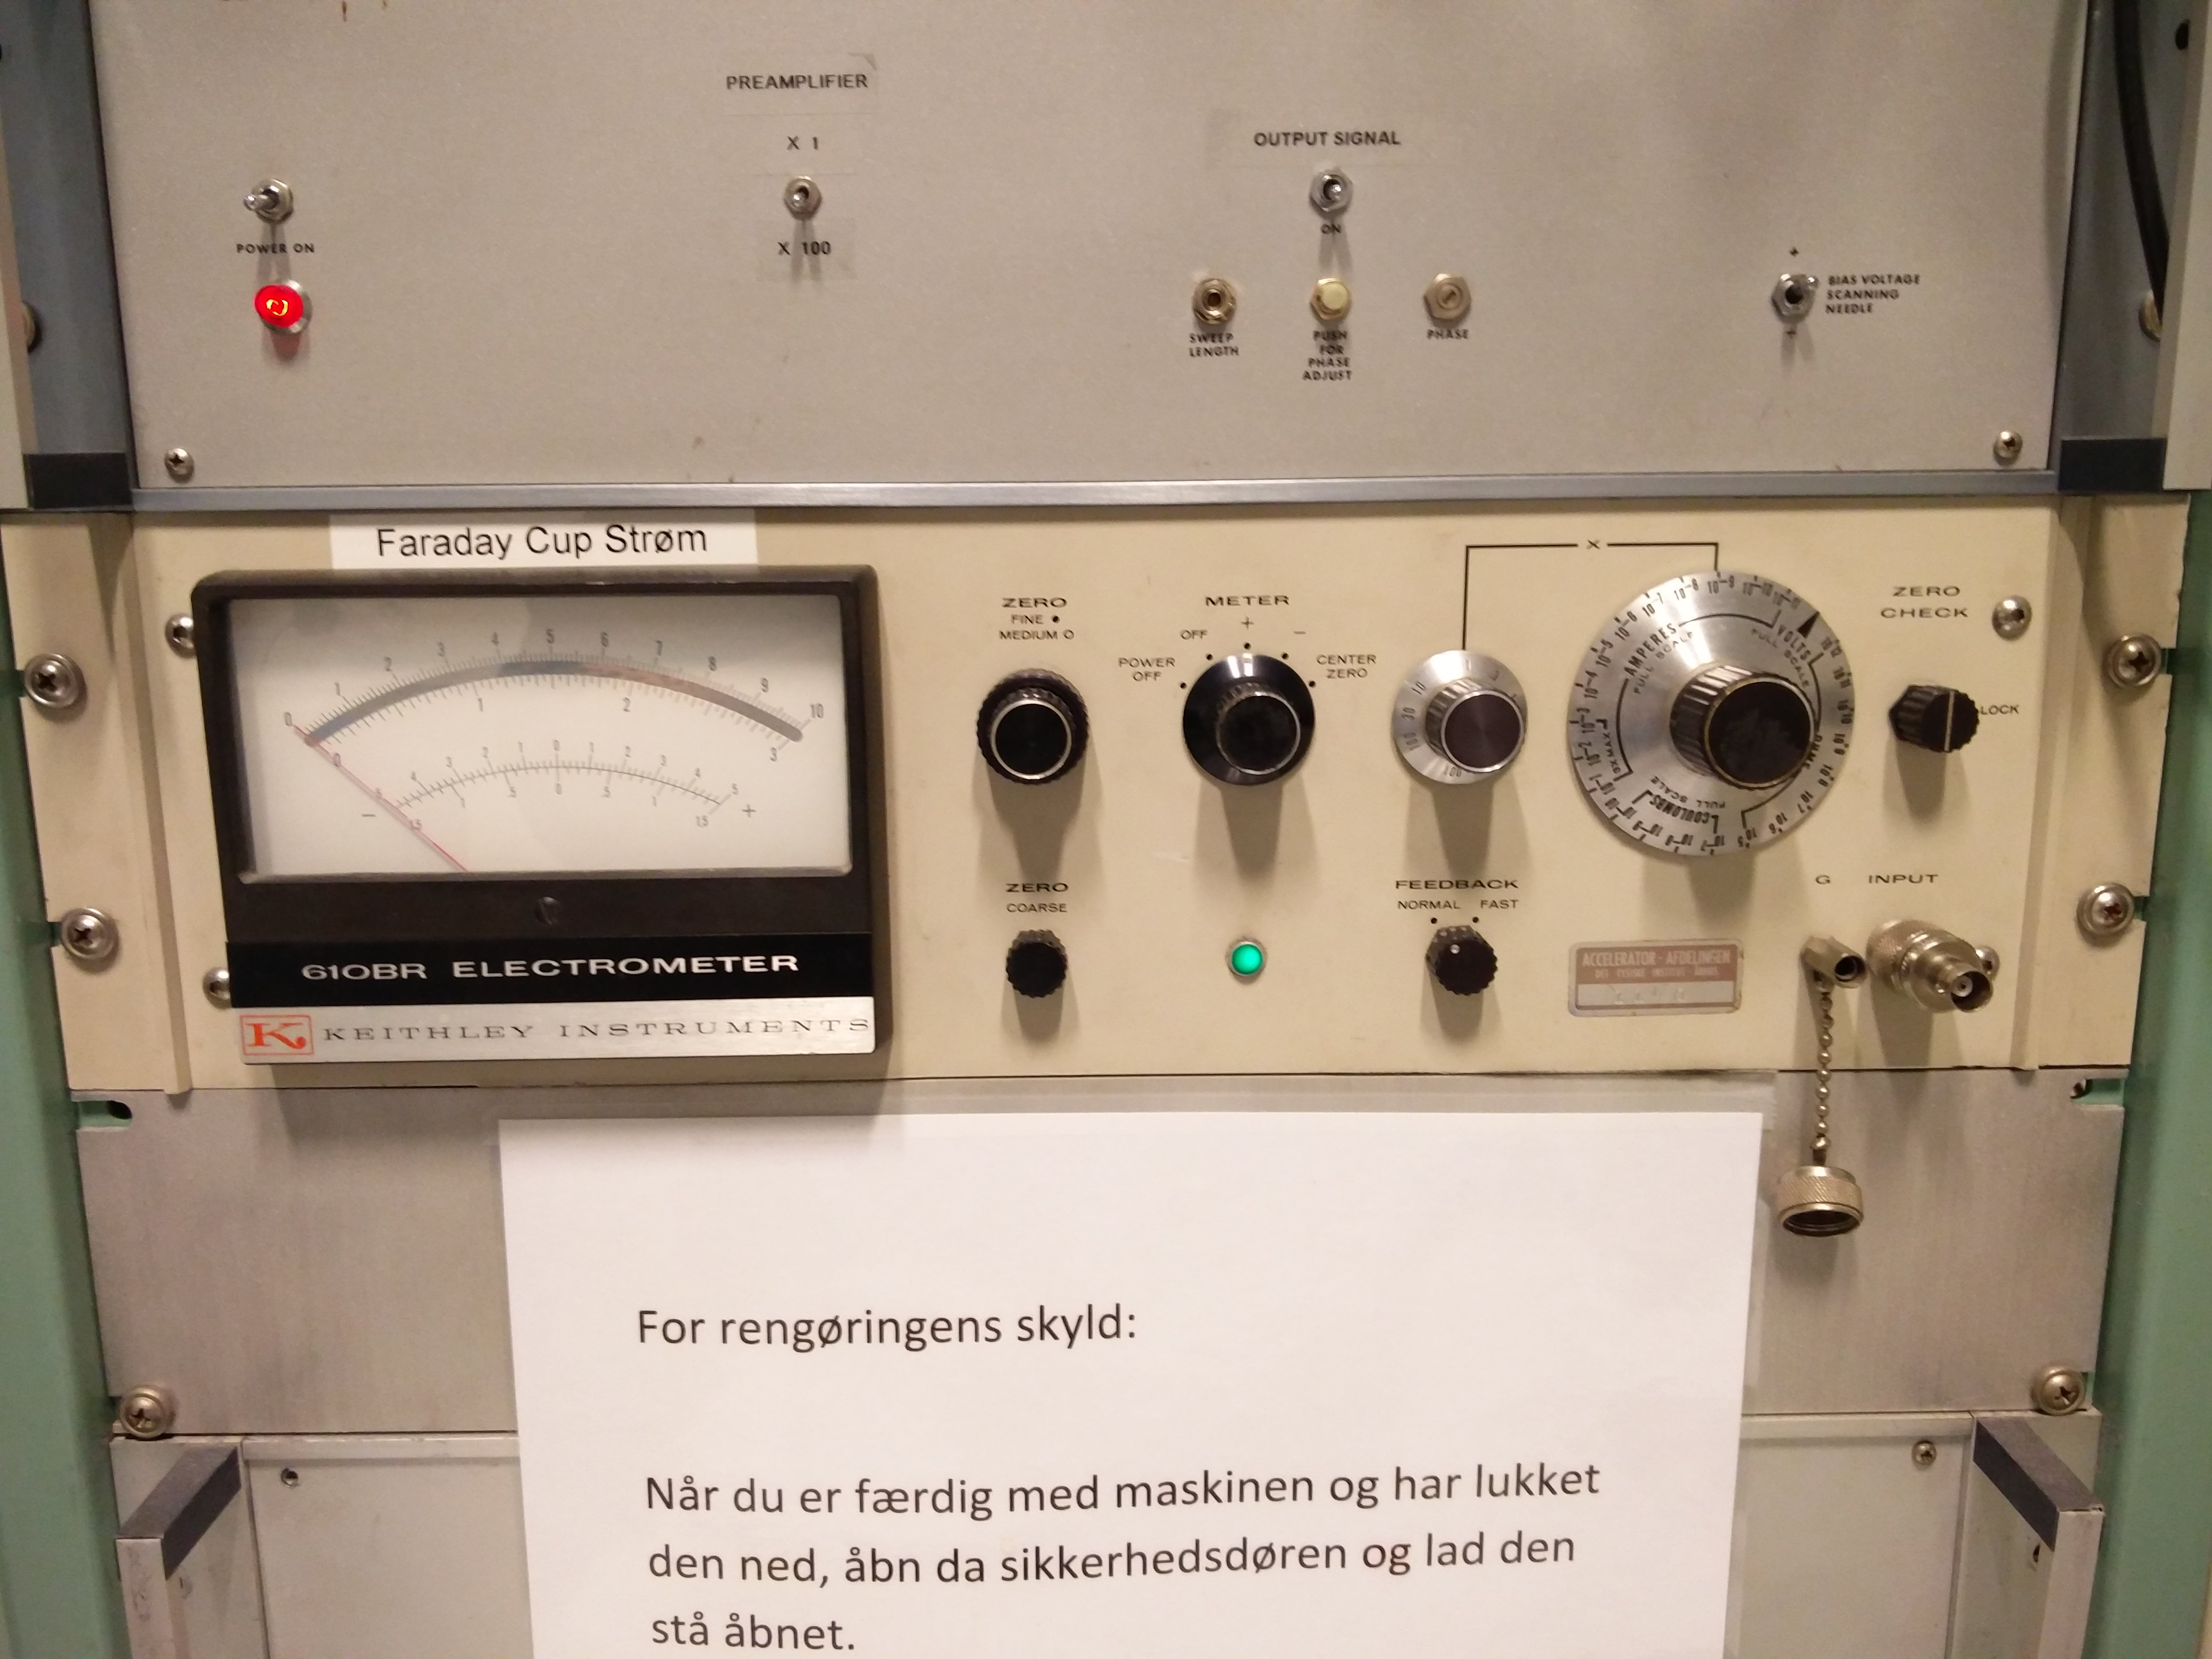
\includegraphics[trim={0, 35cm, 0, 30cm}, clip, width=0.9\columnwidth]{process4}
\caption{Ampere meter connected to the Faraday cup to detect current of charged
particles detected.}
\label{fig_process4}
\end{figure}
When the signal is good, there is one last step which is to set the output of
the faraday cup from the Ampere meter to the input of the collector. This will
give a precise count for the detected ions picked up in the faraday cup.
\begin{figure}[b]
\centering
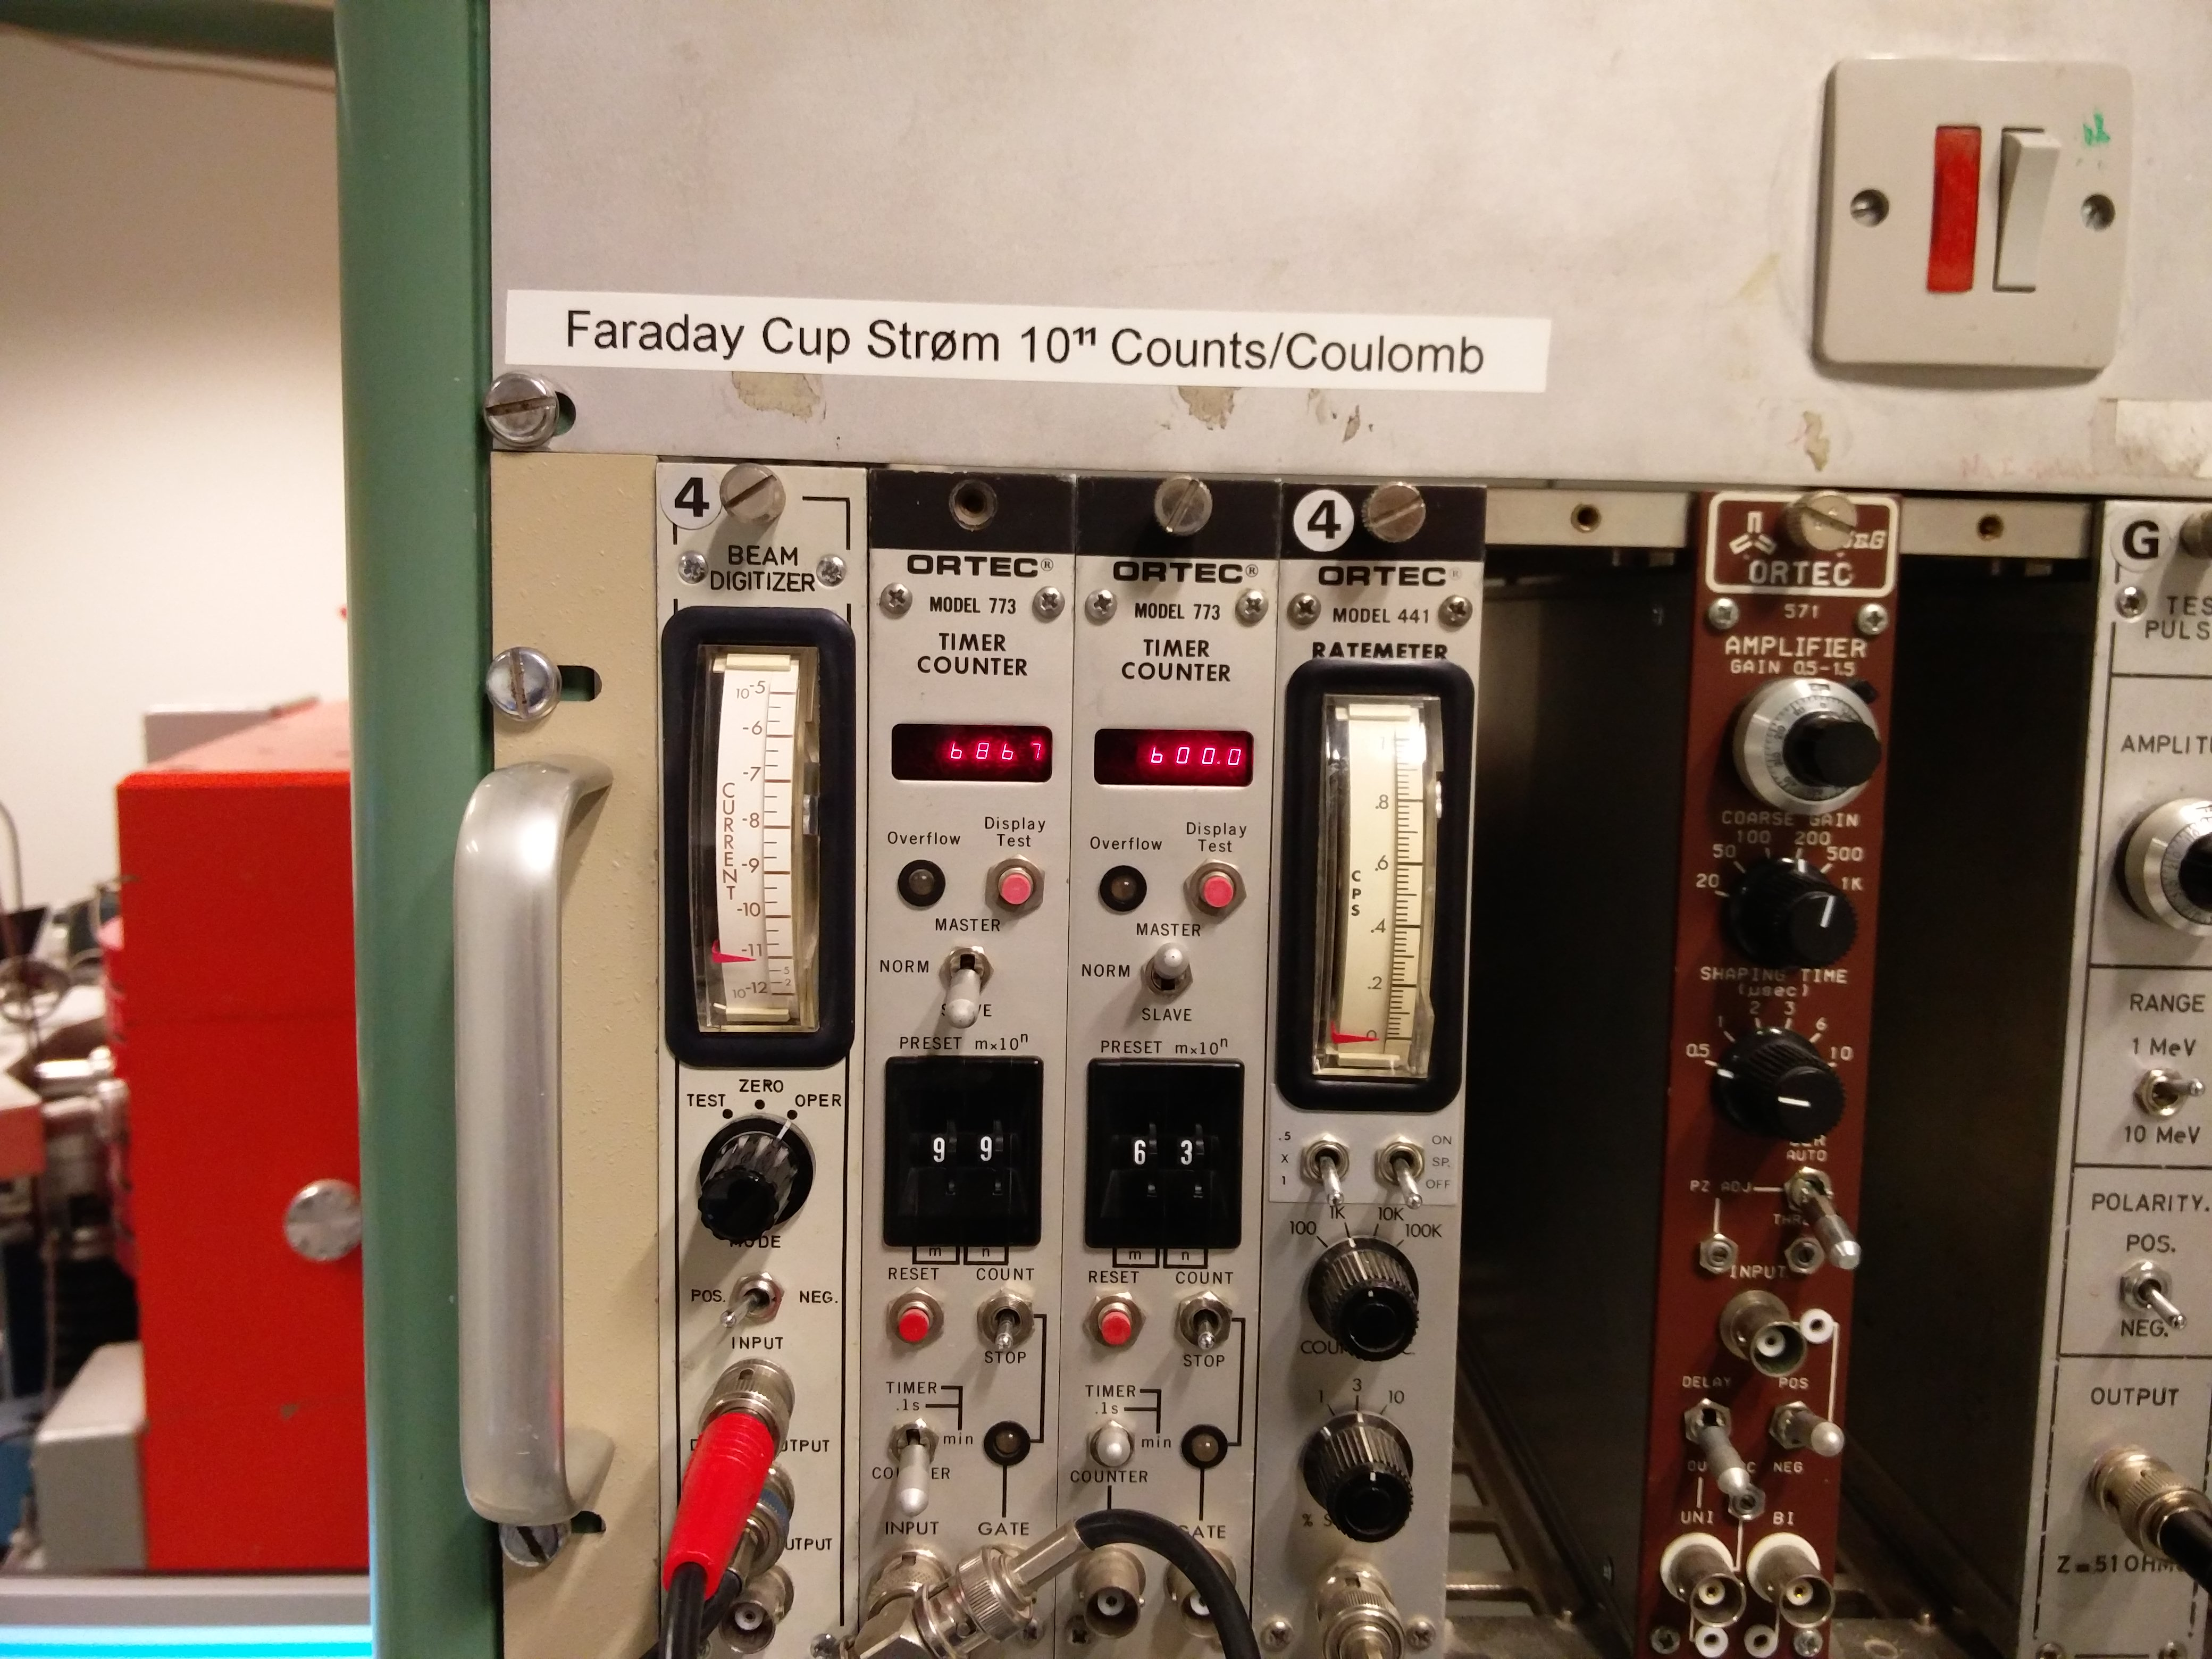
\includegraphics[trim={35cm, 0cm, 0cm, 25cm}, clip, width=0.9\columnwidth]{process5}
\caption{Collector with a timer. This can be set to stop counting after a time
interval.}
\label{fig_process5}
\end{figure}







